%==============================================================================
% tento soubor pouzijte jako zaklad
% this file should be used as a base for the thesis
% Autoři / Authors: 2008 Michal Bidlo, 2019 Jaroslav Dytrych
% Kontakt pro dotazy a připomínky: sablona@fit.vutbr.cz
% Contact for questions and comments: sablona@fit.vutbr.cz
%==============================================================================
% kodovani: UTF-8 (zmena prikazem iconv, recode nebo cstocs)
% encoding: UTF-8 (you can change it by command iconv, recode or cstocs)
%------------------------------------------------------------------------------
% zpracování / processing: make, make pdf, make clean
%==============================================================================
% Soubory, které je nutné upravit nebo smazat: / Files which have to be edited or deleted:
%   projekt-20-literatura-bibliography.bib - literatura / bibliography
%   projekt-01-kapitoly-chapters.tex - obsah práce / the thesis content
%   projekt-01-kapitoly-chapters-en.tex - obsah práce v angličtině / the thesis content in English
%   projekt-30-prilohy-appendices.tex - přílohy / appendices
%   projekt-30-prilohy-appendices-en.tex - přílohy v angličtině / appendices in English
%==============================================================================
\documentclass[slovak,zadani]{fitthesis} % bez zadání - pro začátek práce, aby nebyl problém s překladem
%\documentclass[english]{fitthesis} % without assignment - for the work start to avoid compilation problem
%\documentclass[zadani]{fitthesis} % odevzdani do wisu a/nebo tisk s barevnými odkazy - odkazy jsou barevné
%\documentclass[english,zadani]{fitthesis} % for submission to the IS FIT and/or print with color links - links are color
%\documentclass[zadani,print]{fitthesis} % pro černobílý tisk - odkazy jsou černé
%\documentclass[english,zadani,print]{fitthesis} % for the black and white print - links are black
%\documentclass[zadani,cprint]{fitthesis} % pro barevný tisk - odkazy jsou černé, znak VUT barevný
%\documentclass[english,zadani,cprint]{fitthesis} % for the print - links are black, logo is color
% * Je-li práce psaná v anglickém jazyce, je zapotřebí u třídy použít 
%   parametr english následovně:
%   If thesis is written in English, it is necessary to use 
%   parameter english as follows:
%      \documentclass[english]{fitthesis}
% * Je-li práce psaná ve slovenském jazyce, je zapotřebí u třídy použít 
%   parametr slovak následovně:
%   If the work is written in the Slovak language, it is necessary 
%   to use parameter slovak as follows:
%      \documentclass[slovak]{fitthesis}
% * Je-li práce psaná v anglickém jazyce se slovenským abstraktem apod., 
%   je zapotřebí u třídy použít parametry english a enslovak následovně:
%   If the work is written in English with the Slovak abstract, etc., 
%   it is necessary to use parameters english and enslovak as follows:
%      \documentclass[english,enslovak]{fitthesis}

% Základní balíčky jsou dole v souboru šablony fitthesis.cls
% Basic packages are at the bottom of template file fitthesis.cls
% zde můžeme vložit vlastní balíčky / you can place own packages here

% Kompilace po částech (rychlejší, ale v náhledu nemusí být vše aktuální)
% Compilation piecewise (faster, but not all parts in preview will be up-to-date)
% \usepackage{subfiles}

% Nastavení cesty k obrázkům
% Setting of a path to the pictures
%\graphicspath{{obrazky-figures/}{./obrazky-figures/}}
%\graphicspath{{obrazky-figures/}{../obrazky-figures/}}

%---rm---------------
\renewcommand{\rmdefault}{lmr}%zavede Latin Modern Roman jako rm / set Latin Modern Roman as rm
%---sf---------------
\renewcommand{\sfdefault}{qhv}%zavede TeX Gyre Heros jako sf
%---tt------------
\renewcommand{\ttdefault}{lmtt}% zavede Latin Modern tt jako tt

% vypne funkci šablony, která automaticky nahrazuje uvozovky,
% aby nebyly prováděny nevhodné náhrady v popisech API apod.
% disables function of the template which replaces quotation marks
% to avoid unnecessary replacements in the API descriptions etc.
\csdoublequotesoff

\newtheorem{theorem}{Príklad}[section]
\newtheorem{definition}{Definícia}[section]

\lstdefinestyle{mystyle}{
    backgroundcolor=\color{white},   
    basicstyle=\ttfamily\footnotesize,
    breakatwhitespace=false,         
    breaklines=true,                 
    captionpos=b,                    
    keepspaces=true,                 
    numbers=left,                    
    numbersep=5pt,                  
    showspaces=false,                
    showstringspaces=false,
    showtabs=false,                  
    tabsize=2,
    classoffset = 1,
    frame=single,
    deletekeywords=[2]{input}, 
    keywordstyle=\color{blue},
}

\lstset{style=mystyle}

\usepackage{url}
\usepackage{enumitem}% http://ctan.org/pkg/enumitem
\usepackage{booktabs}% http://ctan.org/pkg/booktabs


% =======================================================================
% balíček "hyperref" vytváří klikací odkazy v pdf, pokud tedy použijeme pdflatex
% problém je, že balíček hyperref musí být uveden jako poslední, takže nemůže
% být v šabloně
% "hyperref" package create clickable links in pdf if you are using pdflatex.
% Problem is that this package have to be introduced as the last one so it 
% can not be placed in the template file.
\ifWis
\ifx\pdfoutput\undefined % nejedeme pod pdflatexem / we are not using pdflatex
\else
  \usepackage{color}
  \usepackage[unicode,colorlinks,hyperindex,plainpages=false,pdftex]{hyperref}
  \definecolor{hrcolor-ref}{RGB}{223,52,30}
  \definecolor{hrcolor-cite}{HTML}{2F8F00}
  \definecolor{hrcolor-urls}{HTML}{092EAB}
  \hypersetup{
	linkcolor=hrcolor-ref,
	citecolor=hrcolor-cite,
	filecolor=magenta,
	urlcolor=hrcolor-urls
  }
  \def\pdfBorderAttrs{/Border [0 0 0] }  % bez okrajů kolem odkazů / without margins around links
  \pdfcompresslevel=9
\fi
\else % pro tisk budou odkazy, na které se dá klikat, černé / for the print clickable links will be black
\ifx\pdfoutput\undefined % nejedeme pod pdflatexem / we are not using pdflatex
\else
  \usepackage{color}
  \usepackage[unicode,colorlinks,hyperindex,plainpages=false,pdftex,urlcolor=black,linkcolor=black,citecolor=black]{hyperref}
  \definecolor{links}{rgb}{0,0,0}
  \definecolor{anchors}{rgb}{0,0,0}
  \def\AnchorColor{anchors}
  \def\LinkColor{links}
  \def\pdfBorderAttrs{/Border [0 0 0] } % bez okrajů kolem odkazů / without margins around links
  \pdfcompresslevel=9
\fi
\fi
% Řešení problému, kdy klikací odkazy na obrázky vedou za obrázek
% This solves the problems with links which leads after the picture
\usepackage[all]{hypcap}

% Informace o práci/projektu / Information about the thesis
%---------------------------------------------------------------------------
\projectinfo{
  %Prace / Thesis
  project={BP},            %typ práce BP/SP/DP/DR  / thesis type (SP = term project)
  year={2021},             % rok odevzdání / year of submission
  date=\today,             % datum odevzdání / submission date
  %Nazev prace / thesis title
  title.cs={Analýza a transformace kódů založená na gramatikách},  % název práce v češtině či slovenštině (dle zadání) / thesis title in czech language (according to assignment)
  title.en={Code Analysis and Transformation Based on Grammars}, % název práce v angličtině / thesis title in english
  %title.length={14.5cm}, % nastavení délky bloku s titulkem pro úpravu zalomení řádku (lze definovat zde nebo níže) / setting the length of a block with a thesis title for adjusting a line break (can be defined here or below)
  %sectitle.length={14.5cm}, % nastavení délky bloku s druhým titulkem pro úpravu zalomení řádku (lze definovat zde nebo níže) / setting the length of a block with a second thesis title for adjusting a line break (can be defined here or below)
  %Autor / Author
  author.name={Matúš},   % jméno autora / author name
  author.surname={Arbet},   % příjmení autora / author surname 
  %author.title.p={Bc.}, % titul před jménem (nepovinné) / title before the name (optional)
  %author.title.a={Ph.D.}, % titul za jménem (nepovinné) / title after the name (optional)
  %Ustav / Department
  department={UIFS}, % doplňte příslušnou zkratku dle ústavu na zadání: UPSY/UIFS/UITS/UPGM / fill in appropriate abbreviation of the department according to assignment: UPSY/UIFS/UITS/UPGM
  % Školitel / supervisor
  supervisor.name={Alexander},   % jméno školitele / supervisor name 
  supervisor.surname={Meduna},   % příjmení školitele / supervisor surname
  supervisor.title.p={prof. RNDr.},   %titul před jménem (nepovinné) / title before the name (optional)
  supervisor.title.a={CSc.},    %titul za jménem (nepovinné) / title after the name (optional)
  % Klíčová slova / keywords
  keywords.cs={konečný automat, zásobníkový automat, rozšírený zásobníkový automat, konfigurácia, gramatika, regulovana gramatika, DNA, RNA, kodón,  aminokyselina, transkripcia, translacia}, % klíčová slova v českém či slovenském jazyce / keywords in czech or slovak language
  keywords.en={finate autmata, pushdown automata, extended pushdown automata, configuration, grammar, regulated grammar, DNA, RNA, codon, amino acid, transcription, translation}, % klíčová slova v anglickém jazyce / keywords in english
  %keywords.en={Here, individual keywords separated by commas will be written in English.},
  % Abstrakt / Abstract
  abstract.cs={Táto práca sa zaoberá analýzou a transformáciou kódu založenej na gramatikách. Práca obsahuje matematicky základ operácii použitých v gramatikách a automatoch. Ich definície, sú sprevádzane príkladmi. V závere je popísaný návrh a implementácia aplikácie, so zameraním na oblasť bioinformatiky, založenej na regulovaných gramatikách. }, % abstrakt v českém či slovenském jazyce / abstract in czech or slovak language
  abstract.en={This thesis is concerning with Code Analysis and Transformation Based on Grammars. The work contains mathematical basics of operations used in grammars and automata.
Their definitions are accompanied by examples.
The design and implementation of the application with focus on the field of bioinformatics, based on regulated grammars is discussed at the end of the theses.
}, % abstrakt v anglickém jazyce / abstract in english
  %abstract.en={An abstract of the work in English will be written in this paragraph.},
  % Prohlášení (u anglicky psané práce anglicky, u slovensky psané práce slovensky) / Declaration (for thesis in english should be in english)
  declaration={Prehlasujem, že som túto bakalársku prácu vypracoval samostatne pod vedením pána prof. RNDr. Alexandra Medunu CSc.
 Uviedol som všetky literárne pramene, publikácie a ďalšie zdroje, z ktorých som čerpal.},
  %declaration={I hereby declare that this Bachelor's thesis was prepared as an original work by the author under the supervision of Mr. X
% The supplementary information was provided by Mr. Y
% I have listed all the literary sources, publications and other sources, which were used during the preparation of this thesis.},
  % Poděkování (nepovinné, nejlépe v jazyce práce) / Acknowledgement (optional, ideally in the language of the thesis)
  acknowledgment={Rád by som sa poďakoval pánovi prof. RNDr. Alexandrovi Medunovi CSc. za jeho odbornú pomoc pri tvorbe tejto práce a jeho cenné rady. Taktiež by som rád poďakoval pani Ing. Ivane Burgetovej Ph.D., za poskytnutie materiálov z oblasti molekulárnej biológie, ktoré poslúžili ako základ práce.},
  %acknowledgment={Here it is possible to express thanks to the supervisor and to the people which provided professional help
%(external submitter, consultant, etc.).},
  % Rozšířený abstrakt (cca 3 normostrany) - lze definovat zde nebo níže / Extended abstract (approximately 3 standard pages) - can be defined here or below
  %extendedabstract={Do tohoto odstavce bude zapsán rozšířený výtah (abstrakt) práce v českém (slovenském) jazyce.},
  %faculty={FIT}, % FIT/FEKT/FSI/FA/FCH/FP/FAST/FAVU/USI/DEF
  faculty.cs={Fakulta informačních technologií}, % Fakulta v češtině - pro využití této položky výše zvolte fakultu DEF / Faculty in Czech - for use of this entry select DEF above
  faculty.en={Faculty of Information Technology}, % Fakulta v angličtině - pro využití této položky výše zvolte fakultu DEF / Faculty in English - for use of this entry select DEF above
  department.cs={Ústav matematiky}, % Ústav v češtině - pro využití této položky výše zvolte ústav DEF nebo jej zakomentujte / Department in Czech - for use of this entry select DEF above or comment it out
  department.en={Institute of Mathematics} % Ústav v angličtině - pro využití této položky výše zvolte ústav DEF nebo jej zakomentujte / Department in English - for use of this entry select DEF above or comment it out
}
% Rozšířený abstrakt (cca 3 normostrany) - lze definovat zde nebo výše / Extended abstract (approximately 3 standard pages) - can be defined here or above
%\extendedabstract{Do tohoto odstavce bude zapsán výtah (abstrakt) práce v českém (slovenském) jazyce.}

% nastavení délky bloku s titulkem pro úpravu zalomení řádku - lze definovat zde nebo výše / setting the length of a block with a thesis title for adjusting a line break - can be defined here or above
%\titlelength{14.5cm}
% nastavení délky bloku s druhým titulkem pro úpravu zalomení řádku - lze definovat zde nebo výše / setting the length of a block with a second thesis title for adjusting a line break - can be defined here or above
%\sectitlelength{14.5cm}

% řeší první/poslední řádek odstavce na předchozí/následující stránce
% solves first/last row of the paragraph on the previous/next page
\clubpenalty=10000
\widowpenalty=10000

% checklist
\newlist{checklist}{itemize}{1}
\setlist[checklist]{label=$\square$}

\begin{document}
  % Vysazeni titulnich stran / Typesetting of the title pages
  % ----------------------------------------------
  \maketitle
  % Obsah
  % ----------------------------------------------
  \setlength{\parskip}{0pt}

  {\hypersetup{hidelinks}\tableofcontents}
  
  % Seznam obrazku a tabulek (pokud prace obsahuje velke mnozstvi obrazku, tak se to hodi)
  % List of figures and list of tables (if the thesis contains a lot of pictures, it is good)
  \ifczech
    \renewcommand\listfigurename{Seznam obrázků}
  \fi
  \ifslovak
    \renewcommand\listfigurename{Zoznam obrázkov}
  \fi
  % {\hypersetup{hidelinks}\listoffigures}
  
  \ifczech
    \renewcommand\listtablename{Seznam tabulek}
  \fi
  \ifslovak
    \renewcommand\listtablename{Zoznam tabuliek}
  \fi
  % {\hypersetup{hidelinks}\listoftables}

  \ifODSAZ
    \setlength{\parskip}{0.5\bigskipamount}
  \else
    \setlength{\parskip}{0pt}
  \fi

  % vynechani stranky v oboustrannem rezimu
  % Skip the page in the two-sided mode
  \iftwoside
    \cleardoublepage
  \fi

  % Text prace / Thesis text
  % ----------------------------------------------
  \ifenglish
    \input{xarbet00-01-kapitoly-chapters-en}
  \else
    % Autor: Matúš Arbet 

\chapter{Úvod}
\label{uvod}

Bioinformatika je relatívne novým, ale rýchlo sa rozvíjajúcim odvetvím. Využíva sa nielen v~biologickom výskume, ale aj pri vývoji liekov, lekárskej diagnostike, poľnohospodárstve a predovšetkým genetike. Hlavnými témami sú vyhľadávanie génov, porovnávanie sekvencií, pravdepodobnosti proteínových štruktúr, vzájomnými vzťahmi medzi génmi. Gény sú základnou zložkou pri tvorbe proteínov, ktoré sú nositeľmi rôznych funkcií buniek organizmov. Gény určujú napríklad farbu vlasov, očí, ale aj hrajú významnú rolu v ľudskom zdraví. Bioinformatika predstavuje tvorbu a vývoj algoritmov, metód a teórií, ktoré riešia problémy pri správe a analýze dát. 

Táto práca sa zaoberá aplikovaním regulovaných gramatík v procese analýzy a prekladu DNA, mRNA sekvencií s cieľom automatizácie a efektívnejšieho riešenia doposiaľ využívaných metód. Jedna zo stávajúcich metód je využitie stochastickej bezkontextovej gramatiky. Tá využíva množinu pravdepodobnosti na produkčných pravidlách. Výpočet pravdepodobnosti derivácie môže byt náročné a môže viesť k nepresnosti výsledkov. Regulované gramatiky sa snažia tento problém redukovať. V práci sa počíta s minimálnou znalosťou danej problematiky, definícií a pojmov, ktoré sú v danej oblasti bežne zaužívané. V jednotlivých kapitolách prace sú definovane pojmy, ktoré na seba postupne nadväzujú a sú nevyhnutné pre pochopenie výrazov a pojmov v nasledujúcej kapitole. 

Teoretická časť práce pozostáva zo štyroch kapitol. V prvej kapitole sú definované základné matematické operácie s ktorými sa budete stretávať v nasledujúcich kapitolách. Prvá kapitola, kde sú tieto pravidlá využívané, je kapitola o bezkontextových gramatikách. Tu sa nachádza definícia bezkontextovej gramatiky, derivácie, generovaného jazyka a neskôr nadväzujúcej regulovanej gramatiky. Pre lepšie pochopenie sú ku každej gramatike priložené príklady, ktoré ukazujú, ako každá gramatika pracuje. V ďalšej kapitole sú definované modely automatov. Tie slúžia, ako základná štruktúra pre popis bezkontextovej gramatiky. Na začiatok je definovaný konečný automat, na ktorý nadväzuje zásobníkový a rozšírený zásobníkový automat. Tie sú vo svojej podstate konečné automaty rozšírené o zásobník, s malými odlišnosťami v procese spracovávania vstupov. Rovnako ako v predošlej kapitole, definície sú sprevádzané príkladmi znázorňujúce princíp fungovania. V závere kapitoly je definovaný regulovaný zásobníkový automat a jeho vzťah so zásobníkovým automatom. Regulovaná gramatika síce nezvyšuje silu pri preklade, v porovnaní s obyčajným zásobníkovým automatom, ale poskytuje jednoduchší a prehľadnejší zápis pravidiel, jeho definovanie a využitie pre účel transformácie DNA, mRNA, ktorými sa tato práca zaoberá. 

V poslednej kapitole teoretickej časti sú prezentované základné pojmy z oblasti molekulárnej biológie. Tie sú nevyhnutne pre pochopenie procesov translácie a transkripcie, ktoré výsledná aplikácia simuluje. Kapitola je sprevádzaná obrázkami, na ktorých sú znázornené prvky DNA, mRNA na úrovni Biochémie. Aj keď sa v práci nezaoberáme jednotlivými atómami molekúl, niektoré pojmy si je zložité predstaviť a môžu byt metúce. Čo je nukleotid, nukleová kyselina, polynukleotidový reťazec, ako to vyzerá, čo sa kde presne na čo viaže a podobne. Taktiež rozdiely medzi DNA a mRNA, proces spracovávania, ich štruktúry sú obsiahnuté v tejto kapitole. Tieto rozdiely sú kľúčovým prvkom v pochopení procesov replikácie, transkripcie a translácie. V akom poradí sa odohrávajú, aký je ich jednotlivý vstup a výstup. Podlá toho je následne možne navrhnúť a definovať automaty v každom procese prekladu DNA, mRNA. Tieto automaty predstavujú základnú štruktúru pre regulovane gramatiky. 

Druhá polovica práce popisuje návrh aplikácie a detailnejšie popisuje implementáciu jednotlivých častí. Implementácia využíva jazyk Python verzia 3.9. Tento jazyk je použitý v implementácií, kvôli jeho vlastnostiam a jednoduchému použitiu. Hlavným pozitívom jazyka v rámci implementácie je napríklad trieda list, ktorá ponuka vlastnosti zásobníku. V tejto kapitole sú definované jednotlivé triedy, automaty a popísaný proces generovania vstupnej sekvencie.





 V závere je spomenuté testovanie aplikácie. To je nevyhnutné v overení správneho fungovania a splnenia požiadaviek, ktoré sú od aplikácie vyžadované. Priebeh testovania prebieha v etapách. V prvej etape testovania je zisťované, či aplikácia zvládne detekovať vstupné chybové zápisy. V ďalšej etape je testované, či aplikácia vykonáva správne operácie pri vstupných parametroch. Tie určujú či aplikácia má vstupnú sekvenciu vygenerovať, prečítať zo súboru, alebo je manuálne zadaná. V závere testovania je nutné jednotlivé časti spojiť v celok a zistiť, či aplikácia dokáže bezchybne vykonávať preklad, ktorý je ešte následne porovnávaný s referenčnou aplikáciou Expasy Traslate Tool\footnote{Dostupná na \href{https://web.expasy.org/translate/}{https://web.expasy.org/translate/}} od Swiss Institute of Bioinformatics.


\chapter{Zakladné matematické pojmy} 
\label{matematika}

V tejto kapitole sú definované matematické pojmy, ktoré sú využité pri definovaní gramatík, pravidiel týchto gramatík, alebo znázornené v demonštračných príkladoch. Definície sú prevzaté z \cite{Automata} a \cite{Mnoziny}. 

\section{Množina}

Množina je súhrn ľubovoľných navzájom rozlíšiteľných objektov. Objekty, ktoré patria do množiny, nazývame prvkami tejto množiny. Množiny obvykle značíme veľkými písmenami a ich prvky malými písmenami latinskej abecedy. Zápis $a \in A$ značí, že $a$ je prvkom množiny $A$. $a \notin A$ značí, že $a$ nie je prvkom množiny $A$. Obvykle ich zapisujeme tak, že do zložených zátvoriek zapíšeme jej jednotlivé prvky alebo pomocou tzv. charakteristických vlastností ako napr.: \{ $x \in \mathbb{N}, 12 < x < 17 $\}, značí množinu tvorenú prvkami 13, 14, 15, 16.

\subsection{Rozdelenie množín} 

\begin{itemize}
\item Konečné -- konečný počet prvkov.
\item Nekonečné -- tvorené nekonečne mnoho prvkami.
\item Prázdne -- neobsahujú žiadny prvok. Značíme ju symbolom $\emptyset$.
\item Neprázdne -- obsahujú aspoň jeden prvok.
\end{itemize}

\subsection{Základné množinové operácie}

\begin{itemize}
\item Zjednotenie $A \cup B$ množín A, B je množina tých prvkov, ktoré patria aspoň do jednej z týchto množín.
\item Prienik $A \cap B$ je množina tých prvkov, ktoré patria do oboch množín súčasne. Ak $A \cap B = \emptyset$, hovoríme, že množiny A, B sú disjunktné.
\item Rozdiel $A - B$ je množina tých prvkov z $A$, ktoré nepatria do množiny $B$. 
\item Doplnok (komplement) $A'$ značí doplnok množiny A tak, že vznikne rozdielom v~nejakej pevne zvolenej množine U tzn. $A' = U - A$.
\item Karteziánsky súčin $A \times B$ množín A, B je množina všetkých usporiadaných dvojíc $[x,y]$, takých kde $x \in A$, $y \in B$.
\end{itemize}

\begin{theorem}
\normalfont Majme množiny $A = \{0, 1, 2\}$, $B = \{-1, 0\}$ a $U = \{a, b\}$. Aplikovaním základných množinových operácii dostávame:
\begin{center}
\item $A \cup B$ = $\{-1, 0, 2\}$
\item $A \cap B$ = $\{0\}$
\item $A - B$ = $\{1, 2\}$
\item $A'$ = $U - A$ = $\{a, b\}$
\item $B \times U = \{-1a, -1b, 0a, 0b \}$
\end{center} 
\end{theorem}

\section{Abeceda a reťazce}

\subsubsection{Abeceda a symboly}
Abeceda je konečná, neprázdna množina elementov, ktoré nazývame symboly. Ak označíme abecedu $\Sigma$, potom $\Sigma$ = $\{a, b, 0, 1\}$ je abeceda obsahujúca symboly a, b, 0, a 1.

\subsubsection{Reťazec}

Nech $\Sigma$ je abeceda.
\begin{enumerate}
\item $\varepsilon$\footnote{Pozn.: $\varepsilon$ označuje prázdny reťazec tzn. neobsahuje žiadny symbol.} je reťazec na abecedou $\Sigma$.
\item Ak $x$ je reťazec nad $\Sigma$ a $a \in \Sigma$, potom $xa$ je reťazec nad abecedou $\Sigma$.
\end{enumerate}

\subsubsection{Dĺžka reťazca}

Nech $x$ je reťazec nad abecedou $\Sigma$. Dĺžka reťazca $x$, $\mid x \mid$, vyjadruje celkový počet symbolov v reťazci $x$ a je definovaná:
\begin{enumerate}
\item Ak $x$ = $\varepsilon$, potom $\mid x \mid$ = $0$.
\item Ak $x$ = $a_1..a_n$, potom $\mid x \mid$ = $n$, pre $n\geq1$ a $a_i \in \Sigma$ pre všetky $i$ = $1,..,n$.
\end{enumerate}

\subsubsection{Konkatenácia reťazcov}

Nech $x$ a $y$ sú dva reťazce nad abecedou $\Sigma$. Konkatenácia $x$ a $y$ je reťazec $xy$\footnote{Pozn.: $\varepsilon$$x = x\varepsilon = x$}.

\subsubsection{Mocnina reťazca}

Nech $x$ je reťazec nad abecedou $\Sigma$. Pre $i\geq0$, i-ta mocnina reťazca $x$, $x^i$, je definovaná:
\begin{enumerate}
\item $x^0$ = $\varepsilon$
\item Pre $x\geq1$ : $x^i = xx^{i-1}$
\end{enumerate}


\begin{theorem}
\normalfont Majme abecedu $\Sigma = \{0, 1\}$. A reťazce $x = 010$ a $y = 1$ nad abecedou $\Sigma$. Nezabúdajme pritom, že aj $\varepsilon$ je reťazcom nad abecedou $\Sigma$. Potom dĺžky zmienených reťazcov sú nasledovné:
\begin{center}
$\mid x \mid$ = $3$,
$\mid y \mid$ = $1$,
$\mid\varepsilon\mid$ = $0$,
\end{center} 

Konkatenáciou reťazcov dostaneme:
\begin{center}
$xy$ = $0101$, $y\varepsilon$ = $1$, $\varepsilon x$ = $010$
\end{center} 

Tretie mocniny reťazcov $x$ a $y$ sú nasledovné:
\begin{center}
$x^3$ = $010010010$, $y^3$ = $111$
\end{center} 
\end{theorem}


\section{Jazyk}

Nech $\Sigma^\ast$ značí množinu všetkých reťazcov nad $\Sigma$. Každá podmnožina $L \subseteq \Sigma^\ast$ je jazyk nad $\Sigma$.

\subsubsection{Konkatenácia jazykov}

Nech $L_1$ a $L_2$ sú dva jazyky nad $\Sigma$. Konkatenácia jazykov $L_1$ a $L_2$, $L_1L_2$ je definovaná:
\begin{center}
$L_1L_2$ = $\{ xy: x \in L_1$ a $y \in L_2 \}$
\end{center}

\subsubsection{Mocnina jazyka}

Nech $L$ je jazyk nad abecedou $\Sigma$. Pre $i\geq0$, i-ta mocnina jazyka $L$, $L^i$, je definovaná:
\begin{enumerate}
\item $L^0$ = $\{\varepsilon\}$
\item Pre $i\geq1$ : $L^i = LL^{i-1}$
\end{enumerate}

\subsubsection{Operácie nad jazykmi}

Nech $L_1$ a $L_2$ sú dva jazyky nad $\Sigma$. Pre ktoré platí: 
\begin{enumerate}
\item Zjednotenie $L_1 \cup L_2$ = $\{ x: x \in L_1$ alebo $x \in L_2 \}$
\item Prienik $L_1 \cap L_2$ = $\{ x: x \in L_1$ a $x \in L_2 \}$
\item Rozdiel $L_1 - L_2$ = $\{ x: x \in L_1$ a $x \not\in L_2 \}$
\end{enumerate}

Ďalej si v úvahe vezmeme jazyk $L$ nad abecedou $\Sigma$. Potom doplnkom jazyka $L$, označovaný $\overline{L}$, je definovaný: 
\begin{center}
$\overline{L}$ = $\Sigma^\ast - L$
\end{center}

\subsubsection{Iterácie jazyka}

Nech $L$ je jazyk nad abecedou $\Sigma$. Iterácia jazyka $L$,$L^\ast$, a pozitívna iterácia jazyka $L$,$L^+$ sú definovane:
\begin{center}
\[ L^\ast = \bigcup_{n=0}^{\infty} L^{i} \]
\[ L^+ = \bigcup_{n=1}^{\infty} L^{i} \]
\end{center}

\begin{theorem}
\normalfont Majme abecedu $\Sigma = \{0, 1\}$ a jazyky $L_1 = \{0, 01\}$ a $L_2 = \{1, 01\}$ nad abecedou $\Sigma$. Predošle definovanými operáciami nad týmito jazykmi dostaneme:
\begin{center}
\item $L_1 \cup L_2$ = $\{0, 1, 01\}$
\item $L_1 \cap L_2$ = $\{01\}$
\item $L_1 - L_2$ = $\{0\}$
\item $L_1L_2$ = $U - A$ = $\{01, 001, 011, 0101\}$
\end{center} 

Ďalej si definujme jazyk $L = \{10, 11\}$ potom:
\begin{center}
\item $\overline{L}$ = $\Sigma^\ast - \{10, 11\}$
\item $L^2$ = $\{1010, 1011, 1110, 1111\}$
\item $L^\ast$ = $\{\varepsilon, 10, 11, 1010, 1011, 1110, 1111, ...\}$
\item $L^+$ = $\{10, 11, 1010, 1011, 1110, 1111, ...\}$
\end{center} 

\end{theorem}

\chapter{Gramatiky}

Bezkontextová gramatika definuje bezkontextový jazyk, ktorého slová sa tvoria nezávisle na predchádzajúcich krokoch. Je tvorená \textit{neterminálmi},  ktoré reprezentujú premenné, \textit{terminálmi}, ktoré reprezentujú konštanty a pravidla. Tie každému \textit{neterminálu} definujú, na čo sa dá prepísať. Bezkontextové gramatiky tvoria neodmysliteľný základ pre pochopenie regulovaných gramatík, ktoré sú na nich založené. Nasledujúca kapitola vychádza z poznatkov knihy \cite{Automata}, ktorá je dobrým úvodom do problematiky. 



\section{Bezkontextová gramatika}
\label{gramatika}

Bezkontextová gramatika je štvorica $G = (N, T, P, S)$, kde:
\begin{itemize}
\item $N$ je abeceda \textit{neterminálov}
\item $T$ je abeceda \textit{terminálov}, kde $N \cap T \neq \emptyset$
\item $P$ je konečná množina pravidiel v tvare $A \to x$, kde $A \in N$, $x \in (N \cup T)^\ast$
\item $S$ je počiatočný symbol, kde $S \in N$ 
\end{itemize} 


Pre používanie gramatík boli zavedené konvencie pre lepšie pochopenie. \textit{Neterminály} sa obvykle zapisujú veľkými písmenami a \textit{terminály} symbolmi, číslicou, alebo malými písmenami. Konečná množina P je v podstate relácia z $N$ do $(N \cup T)^\ast$, ktorú miesto relačného zápisu $(A, x) \in P$ zapisujeme ako $p: A \to x$, kde $p$ značí poradie pravidla v množine. Toto označenie môže byť buď číselné $1, 2, \dots, n$ alebo písmenami malej abecedy s príslušným indexom napr.: $p_1, p_2, \dots, p_n$, kde $n \geq 1$.

\subsection{Priama derivácia}
Nech $G = (N, T, P, S)$ je bezkontextová gramatika, kde $p: A \to w \in P$ a $x, y \in (N \cup T)^\ast$. Potom $xAy$ priamo derivuje $xwy$, ktorú zapíšeme ako $xAy \Rightarrow xwy [p]$, alebo zjednodušene $xAy \Rightarrow xwy$.

\subsection{Sekvencia derivačných krokov}
Majme bezkontextovú gramatiku $G = (N, T, P, S)$, kde $u \in (N \cup T)^\ast$. $G$ vykoná nula derivačných krokov z $u$ do $u$, ktoré zapíšeme:
\begin{center}
$u \Rightarrow^0 u [\varepsilon]$
\end{center} 

zjednodušene:
\begin{center}
$u \Rightarrow^0 u$
\end{center} 

Pre $u_0, \dots, u_n \in (N \cup T)^\ast$ a $p_i \in P$, kde $n \geq 1$, $i = 1, \dots, n$, jednotlivé derivačné kroky vyzerajú nasledovne:
\begin{center}
$u_0 \Rightarrow u_1 [p_1]$
$\Rightarrow u_2 [p_2]$
$\dots$
$\Rightarrow u_n [p_n]$
\end{center} 

Potom $n$-tú deriváciu podľa gramatiky $G$ z $u_0$ do $u_n$ zapisujeme:
\begin{center}
$u_0 \Rightarrow^n u_n [p_1, \dots, p_n]$
\end{center} 

zjednodušene:
\begin{center}
$u_0 \Rightarrow^n u_n$
\end{center}

Matematicky, $\Rightarrow^n$ označuje $n$-tú mocninu $\Rightarrow$. Na základe toho $\Rightarrow^+$ reprezentuje tranzitívny uzáver, ak $n \geq 1$ a $\Rightarrow^\ast$ reflexívny uzáver ak $n \geq 0$.

\subsection{Generovaný jazyk}
Nech $G = (N, T, P, S)$ je bezkontextová gramatika, ak $S \Rightarrow^\ast w$ v $G$. Potom $w$ označuje \textit{vetnú formu}. Ak $w \in T^\ast$, potom $w$ je \textit{veta} generovaná gramatikou $G$. Generovaný jazyk L(G), je množina všetkých viet, ktoré gramatika $G$ generuje a je definovaná:
\begin{center}
$L(G) = \{w: w \in T^\ast, S \Rightarrow^\ast w\}$
\end{center}

\begin{theorem}
\normalfont Majme gramatiku $G = (N, T, P, S)$ a jazyk $L(G) = \{a^nb^n: n \geq 0 \}$, kde:
\begin{itemize}
\item $N = \{S\}$
\item $T = \{a,b\}$
\item $P = \{1: S \to aSb, 2: S \to \varepsilon\}$ 
\end{itemize} 
Gramatika $G$ generuje nasledujúce reťazce:
\begin{flushleft}
\begin{tabular}{p{10em}} 
$S \Rightarrow^\ast \varepsilon$\\
\item $ \quad \Rightarrow^\ast ab [12]$\\
\item $ \quad \Rightarrow^\ast aabb[112]$\\
\item $ \quad \Rightarrow^\ast aaabbb[1112]$\\
\item \quad\quad\quad\vdots
\end{tabular}
\end{flushleft}

\end{theorem}

\section{Regulovaná gramatika}
Regulované gramatiky sú postavené na bezkontextových gramatikách, rozšírené o matematický mechanizmus, ktorým sa kontroluje použitie pravidiel pri generovaní jazyka. Týmto pracujú viac deterministicky než neregulované bezkontextové gramatiky. To zaručuje silnejšiu generatívnu silu. Existujú rôzne typy regulovaných gramatík, ale v tejto práci sa budeme zaoberať len dvoma typmi. Predtým než, ale tak urobíme, potrebujeme poznať odpoveď na otázku: Prečo sa v tejto práci zaoberáme regulovanými gramatikami? V knihe \cite{Methodes} sú popísané metódy molekulárnej biológie v bioinformatike. Kde sa dočítame o použití takzvaných stochastických bezkontextových gramatík. Stochastické bezkontextové gramatiky boli prvý krát použité v kontexte modelovania prirodzeného jazyka. Až neskôr našli svoje uplatnenie v~predikcii sekundárnej štruktúry RNA. Detailnejší popis o tom čo je RNA je venovaná kapitola \ref{biologia}. Stochastická bezkontextová gramatika je takmer rovnako definovaná ako v kapitole \ref{gramatika} s tým rozdielom, že množina pravidiel $P$ je asociovaná s pravdepodobnosťou. Takže zápis $A \to x$ v P vyzerá nasledovne: $Pr(A \to x)$. U stochastických gramatík ale vzniká problém počítania pravdepodobnosti. Toto je riešené zavedením $poľa$ pravidiel a postupnosti. Toto $pole$ pripomína bezkontextovú gramatiku obohatenú o tzv. regulovaný jazyk v regulovaných gramatikách.

\subsection{Stavová gramatika}
Stavová gramatika je bezkontextová gramatika rozšírená o mechanizmus stavov. V derivačnom kroku, gramatika prepisuje najľavejší neterminál a zároveň mení stav, v ktorom sa nachádza a ktorý ovplyvňuje voľbu pravidla použitú v nasledujúcom kroku.
Stavová gramatika je pätica $G = (V, Q\footnote{V knižnej definícii často označované ako $W$, ale kvôli jednotnosti použitého zápisu použijeme označenie $Q$}, T, P, S)$, kde:
\begin{itemize}
\item $V$ je celková \textit{abeceda}
\item $Q$ je konečna množina \textit{stavov}
\item $T \subset V $ je abeceda \textit{terminálov}
\item $S \in V - T$ je \textit{počiatočný neterminál}
\item $P \subseteq (Q \times (V - T)) \times (Q \times V^+)$ je konečna množina \textit{pravidiel}
\end{itemize} 
Používame zápis $(q, A) \to (p, v) \in P$ namiesto zápisu $(q, A, p, v) \in P$. Ak $(q, A) \to (p, v) \in P, x, y \in V^\ast$ tak potom zápis derivačného kroku $(q, xAy)$ do $(q, xvy)$ vyzerá nasledovne: 
\begin{center}
$(q, xAy) \Rightarrow (q, xvy) [(q, A) \to (p, v)]$
\end{center}
$K$-ta mocnina \textit{derivačného kroku} pre $k \geq 0$ je taktiež značená $\Rightarrow^k$. Obnobne sa označuje aj reflexívny $\Rightarrow^\ast$ a tranzitívny $\Rightarrow^+$ uzáver. Potom jazyk generovaný stavovými gramatikami $G$ zapisovaný $L(G)$ je definovaný ako: 
\begin{center}
$L(G) = \{w \in T^\ast \mid (q, S) \Rightarrow^\ast (p, w), q, p \in Q\}$.
\end{center}
\begin{flushleft}
\begin{theorem}
\normalfont Majme stavovú gramatiku $G = (V, Q, T, P, S)$ kde:
\begin{itemize}
\item $V = \{S, A, B, a, b\}$
\item $Q = \{q_1,q_2, p_1, p_2\}$
\item $T = \{a, b\}$
\item $P =$ \begin{tabular}{{ p{12em} p{10em} p{10em} }} 
\vspace{-1,8em}\hspace{1.5em}$ \{ (1.p_1, S) \to (q_1, AB),$ &\vspace{-1,8em}$ (2.q_1, A) \to (q_2,aA),$ &\vspace{-1,8em} $ (3.q_2, B) \to (q_1, bBa), $\\
\vspace{-1,8em}\hspace{2em}$ (4.q_1, A) \to (p_2,a),$ &\vspace{-1,8em} $ (5.p_2, B) \to (p_2, ba)\}$
\end{tabular}
\end{itemize} 
\end{theorem}
\end{flushleft}
Jazyk generovaný gramatikou $G$ je definovaný ako $L(G) = \{a^kb^ka^k, k\geq 1\}$ a jednotlivé derivačne kroky sú nasledovné: 
\begin{center}
\begin{tabular}{p{20em}} 
$(p_1, S) \Rightarrow (q_1, AB) [(1.p_1, S) \to (q_1, AB)]$\\
\item $ \quad\quad\quad\, \Rightarrow (q_2, aAB) [ (2.q_1, A) \to (q_2,aA)]$\\
\item $ \quad\quad\quad\,\Rightarrow (q_1, aAbBa) [ (3.q_2, B) \to (q_1, bBa)]$\\
\item$ \quad\quad\quad\, \Rightarrow (p_2, aabBa) [ (4.q_1, A) \to (p_2,a)]$\\
\item$ \quad\quad\quad\, \Rightarrow (p_2, aabbaa) [(5.p_2, B) \to (p_2, ba)]$
\end{tabular}
\end{center}

\subsection{Gramatika s rozptýleným kontextom}
\label{gramkont}
Gramatika s rozptýleným kontextom $G$ je založená na sekvencií pravidiel bezkontextových gramatík. To umožňuje, aby v jednom derivačnom kroku bolo prepísaných viac \textit{neterminálov} zároveň. Táto gramatika je definovaná ako štvorica $G = (V, T, P, S)$, kde:
\begin{itemize}
\item $V$ je celková \textit{abeceda}
\item $T \subset V $ je abeceda \textit{terminálov}
\item $P$ je konečná množina \textit{pravidiel} vo forme $(A_1, \dots, A_n) \Rightarrow (x_1, \dots, x_n)$, kde $n \geq 1, A_i \in V - T, x_i \in V^\ast$ pre všetky $i$, kde 1 $\geq i \geq n$
\item $S \in V - T$ je \textit{počiatočný neterminál}
\end{itemize} 
$K$-tá mocnina \textit{derivačného kroku} pre $k \geq 0$ je značená ako $\Rightarrow^k_G$, reflexívny $\Rightarrow^\ast_G$ a tranzitívny $\Rightarrow^+_G$ uzáver. Potom jazyk generovaný gramatikou s rozptýleným kontextom $G$ zapisovaný $L(G)$ je definovaný ako: 
\begin{center}
$L(G) = \{w \in T^\ast \mid S \Rightarrow^\ast_G w\}$.
\end{center}
\begin{flushleft}
\begin{theorem}
\normalfont Majme gramatiku s rozptýleným kontextom $G = (V, T, P, S)$ kde: 
\begin{itemize}
\item $V = \{S, A, B, C, a, b, c\}$
\item $T = \{a, b, c\}$
\item $P =\{ (S) \to (ABC), (A, B, C) \to (aAa, bBb, cCc), (A, B, C) \to (a, b, c)\}$
\end{itemize} 
\end{theorem}
\end{flushleft}
Jazyk generovaný gramatikou $G$ je definovaný ako $L(G) = \{a^kb^kc^k, (2K + 1) \geq 0\}$ a jednotlivé derivačne kroky sú nasledovné: 
\begin{center}
\begin{tabular}{p{30em}} 
\quad\,\,$(S) \Rightarrow (ABC) [ (S) \to (ABC) ]$\\
\item $ \quad\quad\quad \Rightarrow (aAabBbcCc) [ (A, B, C) \to (aAa, bBb, cCc)]$\\
\item $ \quad\quad\quad \Rightarrow (aaAaabbBbbccCcc) [ (A, B, C) \to (aAa, bBb, cCc)]$\\
\item$ \quad\quad\quad \Rightarrow (aaaaaabbbbbbcccccc) [ (A, B, C) \to (a, b, c)]$
\end{tabular}
\end{center}




\chapter{Automaty}
Ďalším modelom pre popis bezkontextového jazyka sú automaty. Automat si je možné predstaviť ako zariadenie, ktoré postupnými krokmi v určitej postupnosti, závislosti na vstupnej množine symbolov a množine stavov, rozhodne či je vstupné slovo prijaté, alebo nie. Vstupné slovo je prijaté len vtedy, ak je načítaný celý vstupný reťazec a automat sa nachádza v koncovom stave. Množinu všetkých vstupných slov prijatú automatom tvorí jazyk. Definície automatov sú prevzaté z kníh \cite{Automata}, \cite{Automata2} a \cite{Reggram}.

\section{Konečný automat}
\label{konauto}
Konečný automat je pätica $M = (Q, \Sigma, R, s, F)$, kde:
\begin{itemize}
\item $Q$ je konečná množina \textit{stavov}
\item $\Sigma$ je vstupná \textit{abeceda}
\item $R \subseteq Q \times \Sigma^\ast$\footnote{V knižnej definícii taktiež zaznačené ako $(\Sigma \cup \{\varepsilon\})$}$ \times Q$ je konečná množina \textit{pravidiel}
\item $s \in Q$ je \textit{počiatočný stav}
\item $F \subseteq Q$ je množina \textit{koncových stavov}
\end{itemize} 

Vždy predpokladáme, že množiny $Q$ a $\Sigma$ sú disjunktné tzn. $Q \cap \Sigma = \emptyset$. Používame zápis $pa \to q \in R$ namiesto zápisu $(p, a, q) \in R$. Ak konečný automat $M$ má byť deterministický, znamená to, že $a \neq \varepsilon$. \textit{Konfigurácia} automatu $M$ je každý reťazec $\chi$ z $Q\Sigma^\ast$. Relácia \textit{priameho prechodu} je symbolicky značená $\vdash$ a definovaná ako $pax, qx \in Q\Sigma^\ast, $ ak $ pa \to q \in R$, tak potom:
\begin{center}
$pax \vdash qx$.
\end{center}

$K$-tá mocnina \textit{prechodu} pre $k \geq 0$ je značená $\vdash^k$. Obdobne sa označuje aj reflexívny $\vdash^\ast$ a tranzitívny $\vdash^+$ uzáver. Jazyk prijatý automatom $M$ zapisovaný $L(M)$ je definovaný ako: 
\begin{center}
$L(M) = \{w \in \Sigma^\ast \mid sw \vdash^\ast f, f \in F\}$.
\end{center}
\section{Zásobníkový automat}
Zásobníkový automat je sedmica $M = (Q, \Sigma, \Gamma, R, s, S, F)$, kde:
\label{zasauto}
\begin{itemize}
\item $Q, \Sigma, s$ a $F$ sú rovnako definované, ako v prípade konečného automatu viď. \ref{konauto} 
\item $\Gamma$ je \textit{zásobníková abeceda}
\item $R \subseteq \Gamma \times Q \times \Sigma^\ast \times \Gamma^\ast \times Q$ je konečná množina \textit{pravidiel}
\item $S \in \Gamma$ je \textit{počiatočný symbol} v zásobníku
\end{itemize} 
Taktiež rovnako predpokladáme že možný $Q, \Sigma$ a $\Gamma$ sú disjunktné tzn. $Q \cap \Sigma \cap \Gamma= \emptyset$. Používame zápis $Apa \to wq \in R$ namiesto zápisu $(A, w, p, a, q) \in R$. \textit{Konfigurácia} automatu $M$ je každý reťazec $\chi$ z $Q\Sigma^\ast\Gamma^\ast$. Relácia \textit{priameho prechodu} je rovnako symbolicky značená $\vdash$ a definovaná ako $xApay, xwqy \in Q\Sigma^\ast\Gamma^\ast, $ ak $ Apa \to wq \in R$, tak potom:
\begin{center}
$xApay \vdash xwqy$.
\end{center}
\begin{figure}[!ht]
\centering
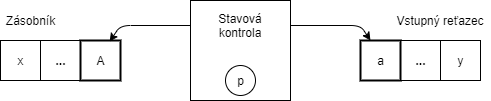
\includegraphics[scale =0.7]{obrazky-figures/automat2.png}
\caption{Znázornenie zásobníkového automatu v stave $p$}
\end{figure}

$K$-tá mocnina \textit{prechodu} pre $k \geq 0$ je taktiež značená $\vdash^k$. Obdobne sa označuje aj reflexívny $\vdash^\ast$ a tranzitívny $\vdash^+$ uzáver. Existujú tri možnosti, v ktorých automat prijme jazyk:
\begin{enumerate}
\item Automat prejde do koncového stavu
\item Vyprázdnením zásobníku
\item Prejdením do koncového stavu a vyprázdnením zásobníku
\end{enumerate}

Jazyk prijatý automatom $M$ pri prechode do koncového stavu, zapisovaný $L(M)_f$ je definovaný ako: 
\begin{center}
$L(M)_f = \{w \in \Sigma^\ast \mid Ssw \vdash^\ast \gamma f, f \in F, \gamma \in \Gamma^\ast\}$.
\end{center}
Jazyk prijatý automatom $M$ vyprázdnením zásobníku, zapisovaný $L(M)_e$ je definovaný ako: 
\begin{center}
$L(M)_e = \{w \in \Sigma^\ast \mid Ssw \vdash^\ast q, q \in Q\}$.
\end{center}
Jazyk prijatý automatom $M$ vyprázdnením zásobníku a prechodom do koncového stavu, zapisovaný $L(M)_{ef}$ je definovaný ako: 
\begin{center}
$L(M)_{ef} = \{w \in \Sigma^\ast \mid Ssw \vdash^\ast f, f \in Fs\}$.
\end{center}



\begin{theorem}
\normalfont Majme zásobníkový automat $M = (Q, \Sigma, \Gamma, R, s, S, F)$. Príjme automat reťazec $accb$? Ak je automat definovaný nasledovne:
\begin{itemize}
\item $Q = \{s, p, q, f\}$
\item $\Sigma = \{a,b, c\}$
\item $\Gamma = \{S\}$
\item $R = \{Ssa \to Sap, apc \to acp, cpc \to q, aqb \to q, Sq \to f\}$ 
\item $F = \{f\}$
\end{itemize} 
Použitím pravidiel z množiny $R$ dostaneme sekvenciu prechodov nasledovnú:
\begin{center}
$Ssaccb \vdash Sapccb \vdash Sacpcb \vdash Saqb \vdash Sq \vdash f$.
\end{center}
Reťazec $accb$ je automatom $M$ prijatý, keďže zásobník automatu je prázdny a zároveň automat prešiel do koncového stavu. Takže platí $accb \in L(M)_{ef}$.
\begin{figure}[!ht]
\centering
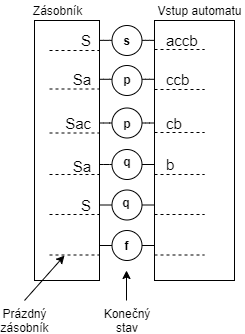
\includegraphics[scale =0.7]{obrazky-figures/schema.png}
\caption{Grafické znázornenie prechodov}
\end{figure}
\end{theorem}




\section{Rozšírený zásobníkový automat}
Rozšírený zásobníkový automat je sedmica $M = (Q, \Sigma, \Gamma, R, s, S, F)$, kde $Q, \Sigma, \Gamma, s, S, F$ sú rovnako definované ako u definícii zásobníkového automatu v predošlej kapitole \ref{zasauto}. Rozdiel je v zápise konečnej množiny pravidiel $R$, ktorá umožňuje čítanie reťazca z vrcholu zásobníku, kde v prípade zásobníkového automatu bolo možne čítanie len jedného symbolu. Toto pravidlo sa zapisuje v tvare: $vpa \to wq$, kde $v, w \in \Gamma^\ast, p, q \in Q, a \in \Sigma^\ast.$ Ak máme dve konfigurácie rozšíreného automatu $xvpay$ a $xwqy$, kde $ x, v, w, \in \Gamma^\ast, p, q \in Q, a, y \in \Sigma^\ast$ pri $vpq \to wq \in R$, potom priamy prechod z $xvpay$ a $xwqy$ pri použití pravidla z množiny $R$ je značený obdobne ako u zásobníkového automatu a vyzerá nasledovne: 
\begin{center}
$xvpay \vdash xwqy$.
\end{center}
Zápis a značenie K-tej mocniny prechodu, tranzitívneho, reflexívneho uzáveru a jazyka prijatého rozšíreným zásobníkovým automatom, zostávajú rovnaké ako u zásobníkového automatu. Pre každý rozšírený zásobníkový automat $M$ existuje zásobníkový automat $M'$, pre ktorý platí $L(M)_f = L(M’)_f$. Dôkaz sa nachádza v knihe \cite{Automata}. 


\section{Regulovaný zásobníkový automat}
\label{regzas}
Regulované zásobníkové automaty sú predstavené v knihe \cite{Reggram}. Vychádzajú z konceptu zásobníkových automatov. Nasledujúca kapitola sa zaoberá zápisom a definovaním regulovaného zásobníkového automatu a prevodu regulovaného zásobníkového automatu regulovaným ľubovoľnou regulovanou gramatikou na zásobníkový automat. Regulovaný zásobníkový automat je dvojica $M_R = (M, \Xi)$, kde:
\begin{itemize}
\item $M = (Q, \Sigma, \Gamma, R, s, S, F) $je zásobníkový automat definovaný ako v kapitole \ref{zasauto},
\item $ \Xi \subseteq \Psi^\ast$ označuje riadiaci jazyk 
\end{itemize} 
Znak $\Psi$ je množina symbolov označenia pravidiel, kde platí, že $card(\Psi) = card(R)$. Potom $\Psi^\ast$ označuje množinu sekvencií všetkých označení pravidiel z $\Psi$. Konfigurácia, prechody a sekvencie zostávajú rovnako definované ako u zásobníkových automatov s rozdielom že musí platiť $r \in \Xi$, kde $r$ reprezentuje sekvenciu použitých pravidiel. Obdobne ako u zásobníkových automatov existujú tri možnosti kedy zásobníkový automat prijme jazyk, tak je tomu rovnako aj v prípade regulovaných zásobníkových automatoch, kedy:
\begin{itemize}
\item $L(M, \Xi, 1)$ jazyk je prijatý ak automat prejde do koncového stavu
\item $L(M, \Xi, 2)$ jazyk je prijatý s vyprázdnením zásobníku
\item $L(M, \Xi, 3)$ jazyk je prijatý ak automat prejde do koncového stavu s vyprázdnením zásobníku
\end{itemize}
Nech $\chi$ je konfigurácia regulovaného zásobníkového automatu $M_R$, kde $\chi \in \Gamma^\ast Q \Sigma^\ast$. Potom koncove konfigurácie pre $i =1, 2, 3,$ sú definované ako:
\begin{enumerate}
\item $\chi \in F$
\item $\chi \in Q$
\item $\chi \in \Gamma^\ast F$ 
\end{enumerate}
Po zavedení koncových konfigurácii automatov, jazyky $L(M, \Xi, i)$ nimi prijaté sú definované nasledovne:
\begin{center}
$L(M, \Xi, i) = \{w \in \Sigma^\ast \mid Ssw \vdash^\ast \chi_i [r], r \in \Xi\}$.
\end{center}
Ak je ale riadiaci jazyk regulárny, tak potom regulovanie automatu riadiacim jazykom nemá žiadny vplyv na jeho generatívnej sile. Dôkaz o tom nájdeme v knihe \cite{Reggram}. Jazyk sekvencie DNA a RNA je regulárny, keďže existuje regulárny výraz, ktorý tento jazyk označuje. Transformáciou na obyčajný zásobníkový automat sa zväčší prehľadnosť zápisu a zjednoduší samotnú implementáciu aplikácie. Transformácia prevedie ľubovoľnú regulárnu gramatiku $G$ a ľubovoľný automat $A$ na obyčajný zásobníkový automat $M$, kde potom platí $L(M) = L(A, L(G), i)$ pri $ i \in {1, 2, 3} $ koncovej konfigurácii automatu. 

\begin{theorem}
\normalfont Majme stavovú gramatiku $G = (V_G, Q_G, T_G, P_G, S_G)$. Zavedením dolného indexu $G$ tak identifikujeme, že $V, Q, T, P$ a $ S$ sú komponentami gramatiky $G$. Obdobne zapíšeme aj automat $A = (Q_A. \Sigma_A, \Gamma_A, R_A, s_A, S_A, F_A)$. Stavová gramatika $G$ je definovaná nasledovne:
\begin{itemize}
\item $V_G = \{S, A, T, U, a, t, u\}$
\item $Q_G = \{s, q_1, q_2, f\}$
\item $T_G = \{a, t, u\}$
\item $P_G = \{1. (s, A) \to (q_1, Sa), 2. (q_1, T) \to (q_2, t), 3. (q_2, U) \to (f, u) \}$
\item $S_G = \{S\}$
\end{itemize} 
Potom automat $A$ je definovaný ako:
\begin{itemize}
\item $Q_A = \{s, q_1, q_2, f\}$
\item $\Sigma_A = \{S, A, T, U\}$
\item $\Gamma_A = \{S, a, t, u\}$
\item $R_A = \{sA \to Saq_1, aq_1T \to tq_2, tq_2U \to uf\}$
\item $s_A = \{s\}$
\item $S_A = \{S\}$
\item $F_A = \{f\}$
\end{itemize} 
Transformáciou na zásobníkový automat $M = (Q_M, \Sigma_M, \Gamma_M, s_M, S_M, F_M, R_M)$ bude definovanie vyzerať nasledovne:
\begin{itemize}
\item $Q_M = \{q \in Q_A\}$
\item $\Sigma_M = \Sigma_A$
\item $\Gamma_M = \Gamma_A$
\item \vspace{-2.5em} $R_M =$ \begin{tabular}{{ p{45em} }} 
\vspace{2em}\hspace{-0.45em}$ \{1.sA \to Saq_1 \in R_A, (s, A) \to (q_1, Sa) \in P_G\} $\\
\hspace{-0.45em}$ \cup \{ 2.aq_1T \to tq_2 \in R_A, (q_1, T) \to (q_2, t) \in P_G\} $ \\
\hspace{-0.45em}$ \cup \{ 3.tq_2U \to uf \in R_A, (q_2, U) \to (f, u) \in P_G \}$
\end{tabular}
\item $s_M = \{s_AS_G\}$
\item $S_M = \{S_A\}$
\item $F_M = \{q \in F_A\}$
\end{itemize} 
\end{theorem}
Uskutočnenie prvého prechodu v zásobníku $M$ je dané pravidlom $1.(s, A) \to (q_1, Sa) \in P_G$ v gramatike $G$. Pri pohľade na pravidla v zásobníku je vidieť, že automat $M$ príjme vstupný reťazec $w$, len ak sa automat $A$ dostane do koncového stavu po prečítaní celého slova $L(G)$, teda platí $L(M) = L(A, L(G), 1)$



\chapter{Molekulárna biológia}
\label{biologia}

Molekulárna biológia je oblasť biológie, ktorá študuje štruktúru, zloženie a vzťahy molekúl buniek, ako napríklad nukleové kyseliny, proteíny, DNA a RNA. Nasledujúca kapitola vychádza z \cite{Bio1}, \cite{Bio2} a \cite{Bio3}.

\section{Bunka}
Bunka patrí medzi základné štruktúry rastlín a živočíchov. Má vlastný metabolizmus, a preto je tento organizmus schopný samostatného života či prenosu genetickej informácie rozmnožovaním. Každá bunka bez ohľadu na funkciu, tvar alebo druh sa skladá z jadra a obalu. Jadro je tvorené cytoplazmou kde prebiehajú metabolické procesy a oblasť ktorá obsahuje genetickú informáciu. Obal je tvorený plazmatickou membránou. Existujú dva typy buniek:
\begin{itemize}
\item Prokaryotická bunka - sú najpočetnejšie na zemi s jednoduchou štruktúrou. Obsahuje prokaryotické jadro (nukleoid) v cytoplazme spolu s deoxyribonukleovou kyselinu. Neobsahuje mitochondrie, plastidy a golgiho aparát. Ich veľkosť sa pohybuje v rozmedzí od $1$ do $10 \mu m$.
\item Eukaryotická bunka - má eukaryotické jadro oddelene od cytoplazmy. Toto jadro obsahuje deoxyribonukleovou kyselinu (DNA), ktorá je nositeľom genetickej informácie. Na rozdiel od prokaryotickej bunky, obsahuje mitochondrie, plastidy a golgiho aparát. Sú niekoľko násobne väčšie od prokaryotickej bunky o veľkosti od $10$ do $100 \mu m$.
\end{itemize} 




\section{Nukleové kyseliny}
Nukleové kyseliny tvoria nevyhnutnú časť každej bunky. Ich hlavnou funkciou je uchovávanie genetickej informácie a jej prenos do dcérskej bunky. Rozlišujeme dva druhy nukleových kyselín:
\begin{itemize}
\item kyselina deoxyribonukleová (DNA)
\item kyselina ribonukleová (RNA)
\end{itemize} 
Obe sa skladajú z troch časti, a to z dusíkatej bázy (zásaditá časť), kyseliny fosforečnej (kyslá časť) a pentózy (cukornatá časť). O tom, o akú kyselinu sa jedná,  rozhoduje sacharid v cukornatej časti. Pre DNA je to deoxyribóza a u RNA ribóza. 
\begin{figure}[!ht]
\centering
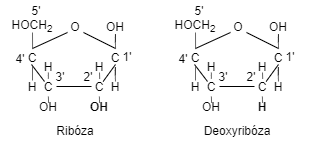
\includegraphics[scale =0.8]{obrazky-figures/riboza2.png}
\caption{Štruktúry pentóz}
\end{figure} 

\newpage

\section{Nukleotidy a polynukleotidový reťazec}
Molekuly nukleotidov sú štruktúrnymi derivátmi buď purínu alebo pyrimidínu. Najbežnejšími purínmi sú adenín (A) a guanín (G). U pyrimidínu je to cytozín (C), uracil (U) a tymín (T). Puríny vytvárajú väzby s pentózou ($5-$uhlíkový cukor) cez svoje $N9$ atómy dusíku, kde u pyrimidínov je to cez $N1$ atómy dusíku. Spojením dusíkatej bázy a pentózy vzniká nukleosid. Ich názvy sú odvodené od dusíkatej bázy, ktorú obsahujú, ako napr.: adenosin, cytidin, uridin a podobne. Ak sa na $5'$ atóm uhlíku pentózy naviaže kyselina fosforečná vzniká nukleotid (adenosinfosfat, uridinfosfat, atď.). Pomocou kyseliny fosforečnej sú jednotlivé nukleotidy pospájané v polynukleotidový reťazec medzi atómami uhlíka $5'$ a $3'$ ribózy, alebo deoxyribozy. Tento reťazec je základom štruktúry nukleových kyselín.
\begin{figure}[!ht]
\centering
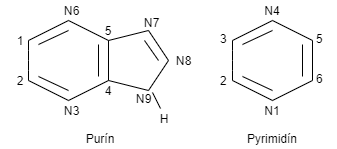
\includegraphics[scale =0.8]{obrazky-figures/purin.png}
\caption{Štruktúry purínu a pyrimidínu}
\end{figure}
\begin{figure}[!ht]
\centering
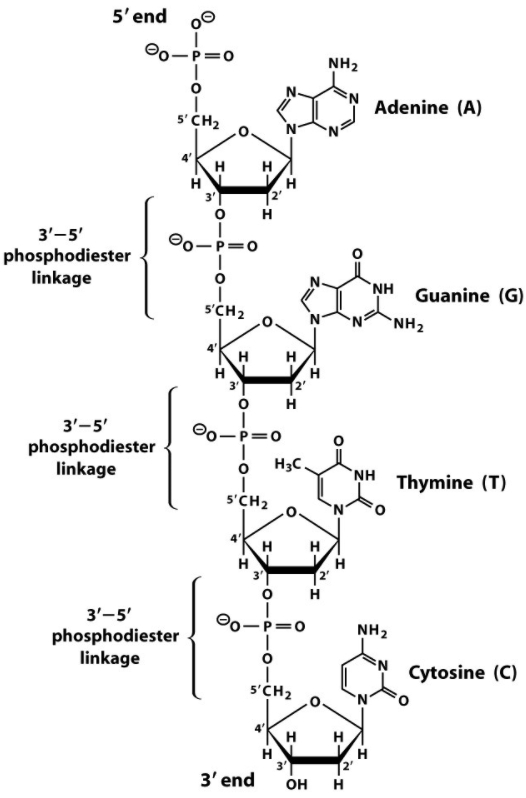
\includegraphics[scale =0.8]{obrazky-figures/polystring.png}
\caption[Príklad polynukleotidového reťazca] {Príklad polynukleotidového reťazca\footnotemark}
\end{figure}





\newpage
\footnotetext{Prevzané z \href{https://sandwalk.blogspot.com/2007/07/dna-is-polynucleotide.html}{https://sandwalk.blogspot.com/2007/07/dna-is-polynucleotide.html}}

\section{Deoxyribonukleová kyselina (DNA)}
\label{vezby}
DNA pozostáva z dvoch komplementárnych vlákien, ktoré formujú tvar tzn. dvojšrúbovice. Tento tvar vzniká pomocou vodíkových väzieb medzi dusíkovými bázami. Tieto bázy môžu obsahovať adenín (A), guanín (G), cytozín (C) a tymín (T). Adenín (A) tvorí pár s tymínom (T) pomocou dvoch vodíkových väzieb (A = T) . Cytozín (C) a guanín (G) tvoria pár pomocou troch vodíkových väzieb (C $\equiv$ G ). Vlákna DNA sú si navzájom antiparalelne, čo znamená, že jedno vlákno je orientovane od $5'$ konca po $3'$ koniec. U druhého je to od konca $3'$ po koniec $5'$. Tieto konce označujú začiatok, koniec a smer polynukleoidového reťazca DNA, v ktorom je uchovaná genetická informácia.

\subsection{Komplementarita}
Princíp komplementárneho párovania báz je základným prvkom DNA štruktúr a má veľký význam v molekulárnej biológii. Párovanie báz je mechanizmus, ktorým je sekvencia molekuly DNA uchovaná počas replikácie, čo je rozhodujúce, ak sa informácia obsiahnutá v géne nesmie zmeniť alebo stratiť počas jej delenia. Ako už bolo spomenuté v predchádzajúcej kapitole \ref{vezby}, adenín (A) sa viaže s tymínom (T) a cytozín (C) s guanínom (G). Nasledujúci príklad popisuje tvorbu komplementárneho plynukleotidoveho reťazca DNA.

\begin{theorem}
\normalfont Majme dva reťazce $A$ a reťazec $B$. Reťazec $A =$ CCATATGGCC, ktorý je orientovaný od $5'$ konca po koniec $3'$. Z tohto reťazca budeme vychádzať a podľa princípov komplementarity nám vznikne príslušný reťazec $B$. Na obrázku \ref{obrkomp} je vidieť, že reťazec $B$ je voči $A$ antiparalelný a reťazec začína koncom $3'$ a konci s $5'$. 
\begin{figure}[!ht]
\centering
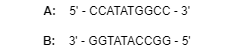
\includegraphics[scale =0.7]{obrazky-figures/kompl.png}
\caption{Komplementárny reťazec $B$ voči reťazcu $A$}
\label{obrkomp}
\end{figure}
\end{theorem}

\subsection{Replikácia}
Replikácia DNA je semikonzervatívna tzn. z každej materskej molekuly DNA vzniknú dve dcérske molekuly DNA. Počas replikácie iba určitá oblasť materskej DNA je rozpletená. Replikácia nastáva po oddelení dvoch vlákien. To zahrňuje rozbitie slabých vodíkových väzieb, ktoré držia bázy protiľahlých vlákien pohromade. Táto oblasť, v ktorej nastane toto oddelenie vlákien sa označuje pod pojmom \textit{replikačná vidlica}. Pre rozdelenie týchto dvoch vlákien sa používa enzým \textit{helikáza}, ktorý zabraňuje ich okamžitému opätovnému spojeniu. Nové väzby s komplementárnym vláknom sú spojené pomocou enzýmu \textit{polymerázy}, ktorý má za úlohu nielen vytvoriť väzby s komplementárnym vláknom, ale aj zabezpečiť to, že replikácia prebehne bez chýb a nová dcérska molekula DNA bude identická k materskej molekule DNA. Syntéza polymerázy prebieha iba v smere od $5'$ konca k $3'$ konca. 

\section{Ribonukleová kyselina(RNA)}
RNA podobne ako DNA obsahuje nukleotidové väzby pomocou fosforečných väzieb. Hlavným rozdielom však je v cukornatej časti, kde sa u RNA nachádza už spomenutá ribóza. RNA pozostáva z jedného vlákna namiesto dvoch, ako v prípade DNA. Ďalší rozdiel je v obsahu zásaditých zložiek, kde je tymín (T) nahradený uracilom (U). Existuje niekoľko druhov RNA. Tie sa rozdeľujú podľa toho či sú nositeľmi genetickej informácie na kodinujúce a nekodinujúce. Medzi kodinujúce patrí mediátorova RNA (mRNA), ktorá je ako jediná nositeľom genetickej informácie. Nekodinujúcich RNA je niekoľko, ale medzi základné patrí transferová RNA (tRNA) a ribozómová RNA (rRNA). 

\subsection{Transkripcia}
Každé molekuly RNA sú kopírované z tzn. DNA šablóny cez proces transkripcie. Proces transkripcie je podobný proces ako replikácia, ale základným rozdielom je dĺžka DNA šablóny použitej pri transkripcii. U replikácii, všetky nukleotidy sú kopírované, kde u transkripcii je použitá iba menšia časť DNA. Je to preto, lebo nie všetky gény sú pri transkripcii potrebné. Šablónou použitou pri tvorbe RNA je jedno vlákno DNA, kde u replikácii DNA boli použité obe vlákna DNA. Počas transkripcie, vzniknutý reťazec RNA je komplementárny a antiparalelný k vláknu DNA šablóny. Tento nový reťazec RNA je taktiež označovaný pod pojmom RNA transkript. Ako enzýmy rozpoznajú, ktorá transkripčná jednotka sa použije, kde začína a kde končí, je zakódované v samotnej DNA sekvencie. Transkripcia je katalyzovaná enzýmom RNA polymerázy, ktorý sa viaže na oblasť promótora a rozpletá časť DNA, označovanú pojmom transkripčná bublina. Promótor je sekvencia DNA indikujúca, ktoré vlákno bude použité ako šablóna a smer, v ktorom bude prebiehať transkripcia. Promótor taktiež určuje začiatok transkripcie. Po vytvorení transkripčnej bubliny, nastáva proces inicializácie, v ktorom je syntetizovaných prvých 9 až 12 nukleotidov RNA. Po skončení inicializácie nastáva proces elongácie. Počas procesu elongácie enzým RNA polymerázy sa už viac neviaže na oblasť promótora, ale pohybuje sa v smere transkripcie po vlákne šablóny DNA a predlžuje RNA reťazec. Koniec transkripcie určuje tzn. terminátor. Je to sekvencia nukleoidov DNA podobná promótoru. V tomto bode sa viac nepokračuje v transkripcii a enzým RNA polymerázy je uvoľnený ako aj výsledný RNA reťazec. Tento reťazec RNA je označovaný ako mediátorova RNA (mRNA). 

\subsection{Translácia}
Translácia sa uskutočňuje na ribozómoch, tie je možné považovať za pohyblivé, proteín syntetizujúce stroje. Ribozóm sa pripája blízko konca $5'$
reťazca mRNA a prekladá sa smerom k $3'$ koncu. Ide o preklad polynukleoidoveho reťazca mRNA do polypeptidového reťazca aminokyselín prostredníctvom genetického kódu. Tento proces sa skladá zo štyroch krokov:
\begin{enumerate}
\item Prvým krokom translácie je väzba molekúl tRNA na príslušné aminokyseliny. Každá tRNA je špecifická pre konkrétnu aminokyselinu. Kľúčom pri špecifikácii medzi aminokyselinou a jej tRNA je enzým aminoacyl-tRNA syntetáza. Bunka má 20 rôznych aminoacyl-tRNA syntetáz, jedna pre každú z 20 aminokyselín. Rozpoznanie tRNA, pomocou enzýmu syntetáz, závisí od rôznych nukleotidových sekvencií tRNA. 
\item Tento krok je nazývaný iniciácia a pozostáva z troch hlavných krokov. Syntéza proteínov sa začína od štart-signálu mRNA AUG kodónu. Najskôr sa mRNA viaže na malú časť ribozómu. Neskôr je iniciačná tRNA naviazaná k mRNA prostredníctvom párovaní báz medzi kodónom a
antikodónom. Nakoniec sa ribozóm pripája k iniciačnému komplexu.
\item Ďalším krokom je elongácia, v ktorej sú aminokyseliny spojené, aby vytvorili polypeptidový reťazec. Ribozóm obsahuje tri väzbové miesta, ktoré môže zabrať tRNA:\begin{itemize}
\item \textit{aminoacyl} nasledovná prichádzajúca aminokyselina vo forme aminoacyl-tRNA
\item \textit{peptidyl} posledná naviazaná aminokyselina vznikajúceho polypeptidového reťazca
\item \textit{exit} alebo \textit{prázdna} predchádzajúca tRNA
\end{itemize} Elongácia prebieha v troch krokoch. V prvom kroku sa tRNA viaže na aminoacylové miesto. Kde sa antikodón tRNA viaže na kodón mRNA. V druhom kroku elongácie sa formuje peptidová väzba medzi aminokyselinami, ktoré sú naviazané na aminoacyl-tRNA miesta. Vytváranie tejto peptidovej väzby uvoľňuje aminokyselinu v peptidylovom mieste od jej tRNA. V tretom kroku sa ribozóm posunie v smere od $5'$ konca do $3'$ konca po mRNA. Ribozóm v tomto kroku je nad novým kodónom a proces elongácie sa môže opakovať.
\item Posledným krokom je terminácia translácie, kde sa na aminoacylové miesto dostaví terminačný kodón. Pretože neexistuje žiadny antikodón komplementárny k terminačnému kodónu, žiadna tRNA sa nenaviaže na aminoacylové miesto. Tieto kodóny sa viažu na tzv. uvoľňovacie faktory, ktoré blokujú naviazanie ďalšej tRNA do aminoacylového miesta a pomáhajú hydrolyzovať väzbu medzi aminokyselinami a tRNA v peptidylovom mieste. Vytvorený polypeptidový reťazec je z ribozómu uvoľnený.
\end{enumerate} 


\section{Bielkoviny}
Bielkoviny sú vo všetkých procesoch organizmov hlavnou zložkou.
Mnohé bielkoviny sú enzýmami (biologickými katalyzátormi), ktoré riadia chemické reakcie buniek. Iné sú štrukturálne
komponenty, ktoré poskytujú podporu pre membrány, vlákna, kosti atď.. Niektoré bielkoviny pomáhajú transportovať látky. Ďalšie majú regulačné, komunikačné,
alebo obranné funkcie. Všetky proteíny sú zložené z aminokyselín, ktoré sú
vzájomne prepojené.

Poznáme $22$ aminokyselín. Ale len $20$ z nich je bielkovinotvorných.
Jedna aminokyselina je kódovaná tromi, po sebe nasledujúcimi nukleotidmi v mRNA. Týmito nukleotidmi môže byť už spomenutý adenín (A), guanín (G), cytozín (C) a uracil (U). Celkovo je teda $64$ kodónov. Tieto kodóny sa nachádzajú v tabuľke \ref{obrgeny}. Tri z týchto kodónov sú stop kodóny, určujúce koniec prekladu.
Každá aminokyselina  pozostáva z atómu uhlíka, naviazaného na aminoskupinu,
atóm vodíka, karboxylová skupina a skupina R (radikál), ktorá sa líši pre každú aminokyselinu. Aminokyseliny v bielkovinách sú
spojené peptidovými väzbami. Rovnako ako nukleové kyseliny majú aj polypeptidy
polaritu, pričom jeden koniec má voľnú aminoskupinu a druhý koniec obsahuje voľnú karboxylovú skupinu.
Niektoré bielkoviny pozostávajú iba z niekoľkých aminokyselín, zatiaľ čo
iné sa môžu skladať z tisícok.

Štruktúra bielkovín rovnako ako v prípade nukleových kyselín, má niekoľko úrovní organizácie.
Primárnou štruktúrou bielkovín je jeho aminokyselinová sekvencia
kyseliny. Interakciami medzi susednými aminokyselinami, polypeptidový reťazec sa prekladá a krúti
do sekundárnej štruktúry. Sekundárne štruktúry
sa skladajú, aby vytvorili terciárnu štruktúru. Nakoniec niektoré bielkoviny, obsahujúce dve a viac polypeptidových reťazcov, vytvoria kvartérnu štruktúru.
\newpage
\begin{figure}[!ht]
\centering
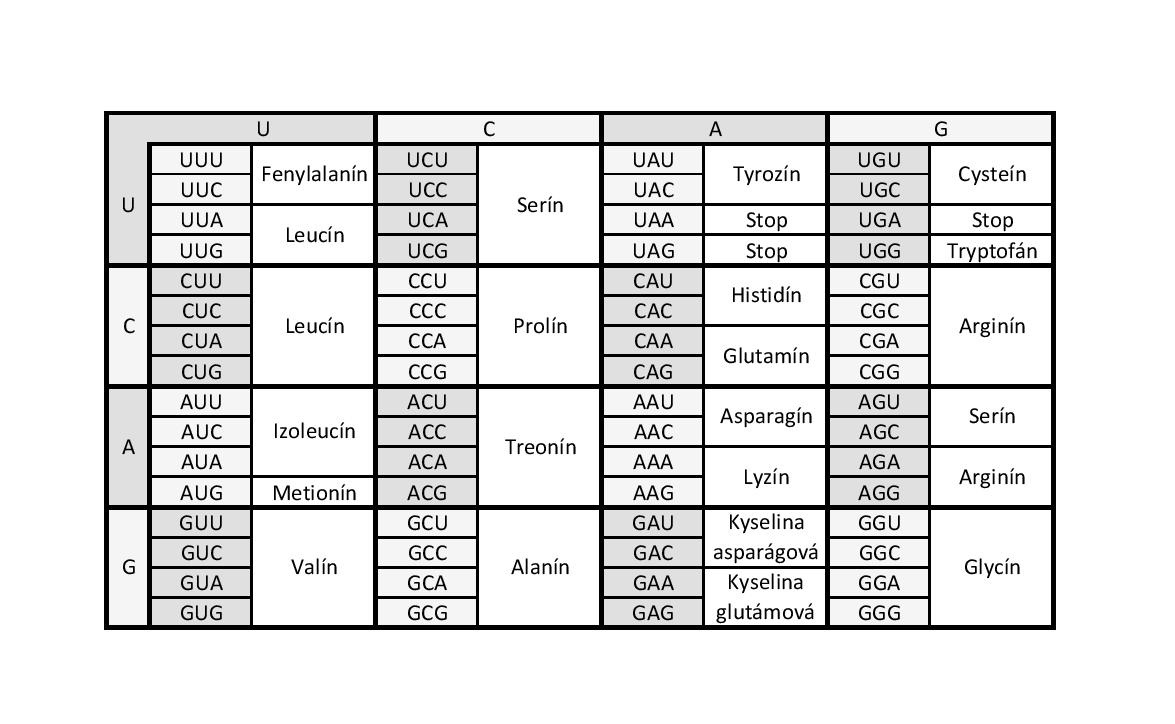
\includegraphics[scale =0.8]{obrazky-figures/geny02.jpg}
\caption{Zoznam aminokyselín a kodónov}
\label{obrgeny}
\end{figure}


\section{Univerzálny štandardizovaný formát}
Textový formát používaný v bioinformatike a biochémii je označovaný ako FASTA formát. Tento formát sa využíva pre reprezentovanie nukleových sekvencií alebo sekvencií aminokyselín. Sekvencia začína jednoriadkovým popisom, za ktorým nasledujú riadky sekvencie dát. Popisný riadok musí vždy začínať symbolom '>' a môže mu predchádzať riadok s komentárom začínajúci symbolom ';'. Riadky sekvencie dát by nemali presiahnuť dĺžku viac ako 80 znakov a musia byť zadané v IBU/IUPAC štandardných kódoch. Tie môžu byť zapísane malými alebo veľkými písmenami latinskej abecedy. Súbory, do ktorých je možné tieto sekvencie uložiť, majú viacero prípon, ktoré značia čo za informáciu je v nich uložená. Medzi základne patria:
\begin{itemize}
\item .fasta, .fa: ľubovoľný druh sekvencie
\item .fna: sekvencia nukleových kyselín
\item .faa: sekvencia aminokyselín
\end{itemize}
FASTA formát môže taktiež obsahovať špeciálne identifikátory. Tieto identifikátory definuje NCBI (National Center for Biotechnology Information), ktoré slúžia ako označenie referencie k záznamu v databáze. Tieto identifikátory nie sú podporované aplikáciou v práci, ale nájdete ich na \cite{FastaID}.


\chapter{Implementácia}

\section{Návrh}
\label{navrh}
Cieľom tejto práce je navrhnúť a implementovať aplikáciu pre prevod DNA a mRNA sekvencii na sekvencie proteínov reprezentované formou reťazcov aminokyselín. Jazyk zvolený pre implementáciu aplikácie je objektovo orientovaný \texttt{Python 3.9}\footnote{Python 3.9 - dokumentacia \href{https://docs.python.org/release/3.9.0/}{https://docs.python.org/release/3.9.0/}}. Pre vývoj aplikácie bol použitý program \texttt{PyCharm}\footnote{PyCharm Python IDE - dostupný na \href{https://www.jetbrains.com/pycharm/}{https://www.jetbrains.com/pycharm/} }. Aplikácia je realizovaná pre operačný systém Linux a Windows.

Vzhľadom na to, že aplikácia má realizovať využitie regulovaných gramatík v odvetví Bioinformatiky a pre pripadne rozšírenia požitia a funkcionality aplikácie, je zbytočné implementovať užívateľské rozhranie. Dôležitá je funkčnosť a použiteľnosť aplikácie. Preto bola zvolená pre implementáciu konzolová aplikácia pre jednoduché zobrazenie výsledkov a interakciu s užívateľom. 
Užívateľ aplikácie je schopný si vstupnú sekvenciu aj vygenerovať. Proces, akým je sekvencia generovaná, je popísaný v sekcii \ref{gener}. Aplikácia je schopná rozoznať o aký typ vstupnej sekvencie sa jedná, ak bola zadaná manuálne, alebo zo súboru a uskutočniť jej preklad. Ten spočíva vo využití troch automatov. Prvý automat $M1$ slúži ako lexikálny analyzátor, vykonávajúci validáciu vstupnej sekvencie ako aj určenie o aký typ vstupnej sekvencie sa jedná (DNA alebo mRNA). Keďže nie je potrebné v tomto kroku využívať zásobník, je využitý konečný automat. Druhý automat $M2$ je využívaný v procese transkripcie. Tento automat je realizovaný ako zásobníkový automat regulovaný stavovou gramatikou. Automat $M3$ vykonáva proces translácie a je realizovaný ako rozšírený zásobníkový automat, regulovaný gramatikou s rozptýleným kontextom. Viac o tom prečo boli zvolené práve tieto gramatiky, sa dozviete v kapitole \ref{automat}.
\section{Triedy aplikácie}
V nasledujúcej sekcii sa nachádza popis jednotlivých tried implementovaných v aplikácii. Každá časť obsahuje stručný výpis kódu, ktorý obsahuje prototyp metód a jednotlivé premenné. Celkovo v aplikácií je definovaných päť tried.

\subsection{Trieda Stack}
\label{stack}
Trieda \texttt{Stack} reprezentuje abstraktnú implementáciu zásobníku. Metódy triedy umožňujú podporu operácii nad zásobníkom, ktorých význam je nasledovný:
\begin{itemize}
\item \texttt{init} - konštruktor vytvárajúci prázdny zásobník
\item \texttt{isEmpty} - zistí, či je zásobník prázdny
\item \texttt{push} - pridá prvok na vrchol zásobníku
\item \texttt{pop} - odoberie prvok z vrcholu zásobníku
\item \texttt{size} - vráti počet prvkov v zásobníku
\item \texttt{top} - vráti prvok nachádzajúci sa na vrchole zásobníku
\end{itemize} 
\begin{lstlisting}[language=Python, caption=Metódy triedy \texttt{Stack}]
class Stack:
def __init__(self):
def isEmpty(self):
def push(self, item):
def pop(self):
def size(self):
def top(self):
\end{lstlisting}

\subsection{Trieda Sequence}
Trieda \texttt{Sequence} reprezentuje vstupnú sekvenciu, ktorá je ďalej spracovaná automatmi. Premenná \texttt{code} obsahuje reťazec vstupnej sekvencie. Typ vstupnej sekvencie je získaný z výstupu automatu $M1$. Ak vstupná sekvencia je validnou DNA, alebo mRNA, tak sa po spracovaní automatom $M2$ zapíše do premenných \texttt{start\_kodon}, \texttt{stop\_kodon} informácia o pozícii štart, a stop kordónov sekvencií. Ak sa jedná o DNA tak to premennej \texttt{transcription} je uložená mRNA získaná z transkripcie. Keďže vstupná sekvencia môže obsahovať viac preložiteľných sekvencii, premenná \texttt{s\_array} slúži pre zápis týchto sekvencii. Podobne aj premenná \texttt{amino} slúži pre uchovanie, ale už aminokyselín získaných z translácie sekvencií z \texttt{s\_array}. Metóda \texttt{getSequence} ukladá do týchto dvoch premenných sekvencie získané zo zásobníka a zároveň odstráni nežiadúce symboly ako štart(S) a stop symbol($\#$). 

\begin{lstlisting}[language=Python, caption=Metódy a premenné triedy \texttt{Sequence}]
class Sequence:
code;
start_kodon;
stop_kodon;
type;
transcription;
s_array;
amino;
def getSequence(self, stack, destination):
\end{lstlisting}

\subsection{Triedy automatov}
Každý automat aplikácie má vlastnú triedu. Triedy \texttt{AutomataM2} a \texttt{AutomataM3} pre svoju funkčnosť pracujú s inštanciou triedy \texttt{Stack}(\ref{stack}). Keďže automat $M1$ je konečný, neobsahuje \texttt{stack}. Premenná \texttt{input} je rovnaká pre všetky automaty. Slúži ako vstup pre automat. Na tento vstup je privedený \texttt{code} objektu triedy \texttt{Sequence}. Premenná \texttt{state} slúži pre ukladanie stavu automatu, v ktorom sa nachádza. Premenná \texttt{top} označuje symbol, ktorý sa momentálne nachádza na vrchole zásobníka. 
\begin{lstlisting}[language=Python, caption=Premenné triedy \texttt{AutomataM1}]
class AutomataM1:
input;
state;
\end{lstlisting}

\begin{lstlisting}[language=Python, caption=Premenné triedy \texttt{AutomataM2}]
class AutomataM2(Stack):
input;
state;
stack;
top;
\end{lstlisting}

\begin{lstlisting}[language=Python, caption=Premenné triedy \texttt{AutomataM3}]
class AutomataM3(Stack):
input;
stack;
top;
\end{lstlisting}

\section{Automaty aplikácie}
\label{automat}
Aplikácia využíva tri automaty. Ako už bolo spomenuté v návrhu \ref{navrh}. Každý z automatov plní odlišnú funkciu vo fázach prekladu vstupnej sekvencie. Týmito fázami sú:
\begin{enumerate}
\item lexikálna analýza - validácia symbolov vstupnej sekvencie
\item transkripcia - preklad DNA sekvencie do mRNA
\item translácia - preklad sekvencie mRNA do reťazca aminokyselín
\end{enumerate} 
\subsection{Automat $M1$}
V procese lexikálnej analýzy prebieha ku klasifikácii sekvencie vstupných symbolov. K tomu nám dobre poslúži konečný automat. Ten vstupnú sekvenciu prejdením do koncového stavu  označí za validnú, ak zodpovedá pravidlám definovaným v množine pravidiel automatu. V~opačnom prípade sekvenciu označí ako chybnú a preklad skončí s príslušnou chybovou hláškou. Konečný automat $M1 = (Q_1, \Sigma_1, R_1, s, F_1)$ je definovaný nasledovne:
\begin{itemize}
\item $Q_1$ = \{$s, u, t, (f$, (INPUT\_ERR | DNA\_OK | DNA\_NOK | mRNA\_NOK | mRNA\_OK))\},
\item $\Sigma_1 \hspace{0.4mm}= \Sigma \cup x,$ kde $x \in \Sigma'$ pričom platí $\Sigma \cap x = \emptyset $,
\item $\Sigma \hspace{2mm}= \{A, C, G, U, T, \#\}$,
\item $R_1 \hspace{0.8mm} = \{ 1.sA \to s, 2.sC \to s, 3.sG \to s, 4.sT \to t, 5.sU \to u, 6.uA \to u, 7.uC \to u, 8.s\# \to (f, $ INPUT\_ERR$), 9.uG \to u, 10.uU \to u, 11.tA \to t, 12.tC \to t, 13.tG \to t, 14.tT \to t, 15.u\# \to (f, $ mRNA\_OK$), 16.uT \to (f, $ mRNA\_NOK$), 17.t\# \to (f, $ DNA\_OK$), 18.tU \to (f, $ DNA\_NOK$), 19.sx \to (f, $ INPUT\_ERR$), 20.ux \to (f, $ INPUT\_ERR$), 21.tx \to (f, $ INPUT\_ERR$)\}$,
\item $s \in Q_1$,
\item $F_1 \hspace{0.8mm}$=~\{($f$, (INPUT\_ERR | DNA\_OK | DNA\_NOK | mRNA\_NOK | mRNA\_OK))\}
\end{itemize} 
Algoritmus \ref{algoritmus1} popisuje kroky realizované automatom $M1$. Ak sa automat dostane do koncového stavu $f$, na tento stav sú viazané signály indikujúce výsledný typ vstupnej sekvencie, ktorých význam je nasledovný:
\begin{itemize}
\item INPUT\_ERR - vo vstupnej sekvencii sa nachádza nevalidný symbol 
\item DNA\_OK - sekvencia na vstupe je validnou DNA
\item DNA\_NOK - vo vstupnej sekvencii sa nachádza chybný výskyt uracilu
\item mRNA\_OK - sekvencia na vstupe je validnou mRNA
\item mRNA\_NOK - vo vstupnej sekvencii sa nachádza chybný výskyt tymínu
\end{itemize} 
\begin{figure}[!ht]
\centering
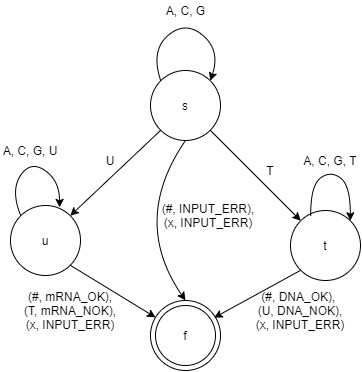
\includegraphics[scale =0.7]{obrazky-figures/M1.jpg}
\caption{Diagram automatu $M1$}
\label{M1obr}
\end{figure}

\begin{algorithm}[H]
\label{algoritmus1}
\SetAlgoLined
\KwResult{Sequence}
\MyStruct{AutomataM1}{
input\;
state; 
}
\MyStruct{Sequence}{
code\;
type\;
\hspace{3mm}\vdots 
}
AutmataM1.input = Sequence.code\;
AutmataM1.input = += '\#'; \tcp{zarážka}
\For{symbol in AutmataM1.input} {
\uIf{(symbol == x) or (symbol == '\#' and stav == 's')}{ 
prechod do stavu '$f$'\;
Sequence.type = INPUT\_ERR\; 
return Sequence; 
}
\uElseIf{(stav == 't') and (symbol == 'U')}{
prechod do stavu '$f$'\;
Sequence.type = mRNA\_NOK\; 
return Sequence; 
} 
\uElseIf{(stav == 't') and (symbol == '\#')}{
prechod do stavu '$f$'\;
Sequence.type = mRNA\_OK\; 
return Sequence; 
}
\uElseIf{(stav == 'u') and (symbol == 'T')}{
prechod do stavu '$f$'\;
Sequence.type = DNA\_NOK\; 
return Sequence; 
} 
\uElseIf{(stav == 'u') and (symbol == '\#')}{
prechod do stavu '$f$'\;
Sequence.type = DNA\_OK\; 
return Sequence; 
}
\uElseIf{(stav == 's') and (symbol == 'T')}{
prechod do stavu '$t$'\;
} 
\uElseIf{(stav == 's') and (symbol == 'U')}{
prechod do stavu '$u$'\; 
}
\Else{
\tcp{načítaj ďalší symbol a ak sa nachádzame v stave 's' tak musí platiť $symbol \in \{A,C,G\}$, ak sme v stave 'u' tak $symbol \in \{A,C,G,U\}$ a ak sme v stave 't' tak $symbol \in \{A,C,G,T\}$.}
}
}
\caption{Automat $M1$}
\end{algorithm}


\newpage

\subsection{Automat $M2$}
Vo fáze transkripcie prebieha preklad validnej DNA, ktorú automat $M2$ obdrží z výstupu automatu $M1$. Automat $M2$ preloží túto sekvenciu na sekvenciu mRNA. Okrem prekladu sekvencie dochádza k získaniu pozícii štart a stop kodónov, ktoré sú potrebné vo fáze translácie automatom $M3$. Okrem sekvencie DNA, automat $M2$ môže prijať aj sekvenciu mRNA. Tá sa už síce neprekladá, ale sú z nej získané pozície kodónov ak sú prítomné v sekvencii. Pozície kodónov sú dôležitým prvkom, ktoré uľahčia proces translácie, keďže sa nie všetky kodóny v polynukleotidovom reťazci prekladajú. Regulovaný zásobníkový automat $M2 = (Q_2, \Sigma_2, \Gamma_2, R_2, s, S_2, F_2)$ je regulovaný stavovou gramatikou $G$, ktorý je definovaný nasledovne: 
\begin{itemize}
\item $Q_2 = \{s, q_1, q_2, q_3, q_4, q_5, q_6, q_7, q_8, q_9, q_{10}, f\}$,
\item $\Sigma_2 \hspace{0.4mm}= \{A, C, G, U, T, \#\}$,
\item $\Gamma_2 \hspace{0.4mm}= \{A, C, G, U, S, \#\}$,
\item $R_2 \hspace{0.4mm} = R_{21} \cup R_{22} \cup R_{23} \cup R_{24} \cup R_{25} \cup R_{26} \cup R_{27} \cup R_{28} \cup R_{29} \cup R_{210} \cup R_{211} \cup R_{212} \cup R_{213} \cup R_{214} \cup R_{215} \cup R_{216} \cup R_{217} \cup R_{218} \cup R_{219} \cup R_{220} \cup R_{221} \cup R_{222} \cup R_{223} \cup R_{224} \cup R_{225} \cup R_{226} \cup R_{227} \cup R_{228} \cup R_{229}$, kde $R_{2i}, i = <1, 29>, (R_3 - R_{2i}) \cup R_{2i} = \emptyset $ 
\item $s \in Q_2$,
\item $F_2 \hspace{1.8mm}$=~\{$f$\}
\end{itemize} 
Množiny pravidiel $R_{2i},$ pre $i = <1, 18>$, sú obsiahnuté v tabuľke \ref{M2table}. Množiny $R_{2i},$ pre $i = <19, 29>$, obsahujú koncové pravidlá, kedy automat narazí na zarážku. Tie sú v tvare $n.(p, p\#) \to (f, f)$, kde $n = 41 + i$, $p \in (Q_2 - \{f\}), f \in F_2$. 

\begin{figure}[!ht]
\centering
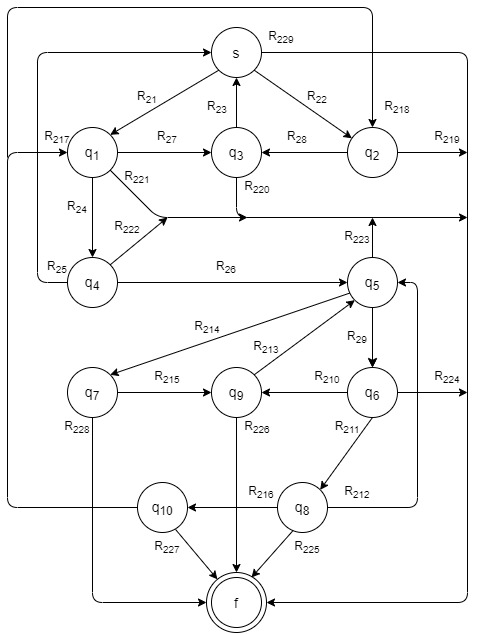
\includegraphics[scale =0.7]{obrazky-figures/M2.jpg}
\caption{Diagram automatu $M2$}
\label{M2obr}
\end{figure}

\newpage

\begin{longtable}{ |p{1.5cm}||p{12.5cm}| }
\hline
\multicolumn{1}{| c ||}{\textbf{Množina}}
& 
\multicolumn{1}{c |}{\textbf{Pravidlá}}\\
\hline
\multicolumn{1}{| c ||}{$R_{21}$} & $1.(s; sA) \to (q_1; Aq_1)$, \\
\hline
\multicolumn{1}{| c ||}{$R_{22}$} & $2.(s; sC) \to (q_2; Cq_2), 3.(s; sT) \to (q_2; Uq_2), 4.(s; sG) \to~(q_2; Gq_2),\newline 5.(s; sU) \to (q_2; Uq_2)$, \\
\hline
\multicolumn{1}{| c ||}{$R_{23}$} & $6.(q_3; q_3A) \to (s; As), 7.(q_3; q_3T) \to (s; Us), 8.(q_3; q_3G) \to~(s; Gs),\newline 9.(q_3; q_3U) \to (s; Us), 10.(q_3; q_3C) \to (s; Cs)$, \\
\hline
\multicolumn{1}{| c ||}{$R_{24}$} & $11.(q_1; Aq_1T) \to (q_4; AUq_4), 12.(q_1; Aq_1U) \to (q_4; AUq_4)$, \\
\hline
\multicolumn{1}{| c ||}{$R_{25}$} & $13.(q_4; q_4A) \to (s; As), 14.(q_4; q_4C) \to (s; Cs), 15.(q_4; q_4T) \to (s; Us), 16.(q_4; q_4U) \to (s; Us)$, \\
\hline
\multicolumn{1}{| c ||}{$R_{26}$} & $17.(q_4; Uq_4G) \to (q_5; UGq_5)$, \\
\hline
\multicolumn{1}{| c ||}{$R_{27}$} & $18.(q_4; Aq_4A) \to (s; AAs), 19.(q_4; Aq_4C) \to (s; ACs), 20.(q_4; Aq_4G) \to (s; AGs)$, \\
\hline
\multicolumn{1}{| c ||}{$R_{28}$} & $21.(q_2; q_2A) \to (q_3; Aq_3), 22.(q_2; q_2T) \to (q_3; Uq_3), 23.(q_2; q_2G) \to (q_3; Gq_3), \newline 24.(q_2; q_2U) \to (q_3; Uq_3), 25.(q_2; q_2C) \to (q_3; Cq_3)$, \\
\hline
\multicolumn{1}{| c ||}{$R_{29}$} & $26.(q_5; q_5T) \to (q_6; Uq_6), 27.(q_5; q_5U) \to (q_6; Uq_6)$, \\
\hline
\multicolumn{1}{| c ||}{$R_{210}$} & $28.(q_6; Uq_6T) \to (q_9; UUq_9), 29.(q_6; Uq_6C) \to (q_9; UCq_9), 30.(q_6; Uq_6U) \to (q_9; UUq_9)$, \\
\hline
\multicolumn{1}{| c ||}{$R_{211}$} & $31.(q_6; Uq_6A) \to (q_8; UAq_8), 32.(q_6; Uq_6G) \to (q_8; UGq_8)$, \\
\hline
\multicolumn{1}{| c ||}{$R_{212}$} & $33.(q_8; Aq_8T) \to (q_5; AUq_5), 34.(q_8; Aq_8C) \to (q_5; ACq_5), 35.(q_8; Aq_8U) \to (q_5; AUq_5), 36.(q_8; Gq_8C) \to (q_5; GCq_5), 37.(q_8; Gq_8U) \to (q_5; GUq_5),\newline 38.(q_8; Gq_8T) \to (q_5; GUq_5)$, \\
\hline
\multicolumn{1}{| c ||}{$R_{213}$} & $39.(q_9; q_9A) \to (q_5; Aq_5), 40.(q_9; q_9T) \to (q_5; Uq_5), 41.(q_9; q_9G) \to (q_5; Gq_5), \newline 42.(q_9; q_9U) \to (q_5; Uq_5), 43.(q_9; q_9C) \to (q_5; Cq_5)$, \\
\hline
\multicolumn{1}{| c ||}{$R_{214}$} & $44.(q_5; q_5A) \to (q_7; Aq_7), 45.(q_5; q_5C) \to (q_7; Cq_7), 46.(q_5; q_5G) \to (q_7; Gq_7)$, \\
\hline
\multicolumn{1}{| c ||}{$R_{215}$} & $47.(q_7; q_7A) \to (q_9; Aq_9), 48.(q_7; q_7T) \to (q_9; Uq_9), 49.(q_7; q_7G) \to (q_9; Gq_9), \newline 50.(q_7; q_7U) \to (q_9; Uq_9), 51.(q_7; q_7C) \to (q_9; Cq_9)$, \\
\hline
\multicolumn{1}{| c ||}{$R_{216}$} & $52.(q_8; Aq_8A) \to (q_{10}; AAq_{10}), 53.(q_8; Aq_8G) \to (q_{10}; AGq_{10}), 54.(q_8; Gq_8A) \newline \to (q_{10}; GAq_{10})$, \\
\hline
\multicolumn{1}{| c ||}{$R_{217}$} & $55.(q_{10}; q_{10}A) \to (q_1; Aq_1)$, \\
\hline
\multicolumn{1}{| c ||}{$R_{218}$} & $56.(q_{10}; q_{10}C) \to (q_2; Cq_2), 57.(q_{10}; q_{10}T) \to (q_2; Uq_2), 58.(q_{10}; q_{10}G) \to \newline(q_2; Gq_2), 59.(q_{10}; q_{10}U) \to (q_2; Uq_2)$, \\
\hline
\caption{Tabuľka množín pravidiel automatu $M2$}
\label{M2table}
\end{longtable}


\subsection{Automat $M3$}
Rozšírený zásobníkový automat $M3$ regulovaný gramatikou s rozptýleným kontextom \ref{gramkont} nám umožňuje v procese translácie, zo vstupnej sekvencie prečítať viac symbolov (nukleotidov) naraz. V procese translácie sú to vždy tri nukleotidy pre každú aminokyselinu. Aby sme boli schopní tieto symboly naraz preložiť, k tomu nám slúži už spomenutá regulovaná gramatika. Proces translácie prebieha nasledovne. Automat $M3$ obdrží z výstupu automatu $M2$ objekt triedy \texttt{Sequence}. Ten obsahuje pozície štart a stop kodónov, ktoré vymedzujú preložiteľné časti vstupnej sekvencie. Automat obsahuje 2 stavy $s, f$. Ten sa pri načítavaní vždy troch symbolov nachádza v stave $s$ pokiaľ nenarazí na zarážku. Použitím pravidla z množiny $R_3$ preloží na príslušnú skratku aminokyseliny, ktorú zapíše na vrchol zásobníka. Skratka príslušnej aminokyseliny pozostáva z prvých troch písmen názvu. Jednotlivé názvy aminokyselín boli spomenuté v tabuľke \ref{obrgeny}. Zarážka $\#$ signalizuje koniec procesu translácie a automat prechádza do koncového stavu $f$. Automat $M3 = (Q_3, \Sigma_3, \Gamma_3, R_3, s, S, F_3)$ je definovaný nasledovne:

\begin{itemize}
\item $Q_3 = \{s, f\}$,
\item $\Sigma_3 \hspace{0.2mm}= \{A, C, G, U, T, S, \#\}$, 
\item $\Gamma_3 \hspace{0.4mm}= \{Phe, Leu, Ile, Met, Val, Ser, Pro, Thr, Ala, Tyr, His, Gln, Ans, Lys, Cys, Trp, \newline Arg, Glu, Asp, Gly\}$, 
\item $R_3$ viz tabuľka \ref{M3table}, 
\item $s \in Q_3$,
\item $F_3 \hspace{1.6mm}$=~\{$f$\}
\end{itemize}


\begin{longtable}{ |p{1.5cm}||p{12.5cm}| }
\hline
\multicolumn{1}{| c ||}{$R_3$}
& 
$1.sUUU \to Phes, 2.sUUC \to Phes, 3.sUUA \to Leus, \newline
4.sUUG \to Leus, 5.sCUU \to Leus, 6.sCUC \to Leus, \newline
7.sCUA \to Leus, 8.sCUG \to Leus, 9.sAUU \to Iles, \newline
10.sAUC \to Iles, 11.sAUA \to Iles, 12.sAUG \to Mets, \newline
13.sGUU \to Vals, 14.sGUC \to Vals, 15.sGUA \to Vals, \newline 
16.sGUG \to Vals, 17.sUCU \to Sers, 18.sUCC \to Sers, \newline 
19.sUCA \to Sers, 20.sUCG \to Sers, 21.sCCU \to Pros, \newline
22.sCCC \to Pros, 23.sCCA \to Pros, 24.sCCG \to Pros, \newline
25.sACU \to Thrs, 26.sACC \to Thrs, 27.sACA \to Thrs, \newline
28.sACG \to Thrs, 26.sGCU \to Alas, 27.sGCC \to Alas, \newline
28.sGCA \to Alas, 29.sGCG \to Alas, 30.sUAU \to Trys, \newline
31.sUAC \to Trys, 32.sCAU \to Hiss, 33.sCAC \to Hiss, \newline
34.sCAA \to Glns, 35.sCAG \to Glns, 36.sAAU \to Anss, \newline
37.sAAC \to Anss, 38.sAAA \to Lyss, 39.sAAG \to Lyss, \newline
40.sUGU \to Cyss, 41.sUGC \to Cyss, 42.sUGG \to Trps, \newline
43.sCGU \to Args, 44.sCGC \to Args, 45.sCGA \to Args, \newline
46.sCGG \to Args, 47.sAGA \to Args, 48.sAGG \to Args, \newline
49.sAGU \to Sers, 50.sAGC \to Sers, 51.sGAU \to Asps, \newline 
52.sGAC \to Asps, 53.sGGU \to Glys, 54.sGGC \to Glys, \newline
55.sGGA \to Glys, 56.sGGG \to Glys, 57.s\# \to f, $ \\
\hline
\caption{Tabuľka pravidiel množiny $R_3$ automatu $M3$}
\label{M3table}
\end{longtable}


\begin{theorem}
\label{prikladsek}
\normalfont Majme vstupnú sekvenciu $x = CTGATGCTTTAA$, ktorá bude vstupom pre automat $M1$. 
Použitím pravidiel z množiny $R_1$ dostaneme sekvenciu prechodov nasledovnú:
\begin{flushleft}
$sCTGATGCTTTAA \vdash sTGATGCTTTAA \vdash tGATGCTTTAA \vdash tATGCTTTAA \vdash tTGCTTTAA \vdash tGCTTTAA
\vdash tCTTTAA \vdash tTTTAA \vdash tTTAA \vdash tTAA \vdash tAA \vdash \newline tA \vdash t\# \vdash f(DNA\_OK) [2, 4, 13, 11, 14, 13, 12, 14, 14, 14, 11, 11, 17] $
\end{flushleft}
Automat prešiel do koncového stavu $f$ so signálom $DNA\_OK$. Indikujúc, že sa jedná o validnú DNA a môže byť ďalej použitá pre vstup automatu $M2$. Ten použitím pravidiel z množiny $R_2$, sekvencia prechodov automatu je nasledovná:
\begin{flushleft}
$SsC \vdash Cq_2T \vdash Uq_3G \vdash GsA \vdash Aq_1T \vdash AUq_4G \vdash UGq_5C \vdash GCq_7T \vdash CUq_9T \vdash UUq_5T \vdash UUq_6A \vdash UAq_8A \vdash AAq_{10}\# \vdash f [2, 22, 8, 1, 11, 17, 45, 48, 40, 26, 31, 52, 68] $
\end{flushleft}
Výstupná sekvencia CUGAUGCUUUAA automatu $M2$ je uložená na zásobníku. Ak pri aplikovaní pravidiel, automat využije postupne za sebou pravidlá z množín $R_{21}, R_{24} a R_{26}$, automat narazil na štart kodón sekvencie. V tomto príklade sa jedná o pravidlá $1, 11 a 17$. Pozícia štart kodónu sa uloží do príslušnej premennej objektu triedy \texttt{Sequence}. Obdobne to platí pre pozíciu stop kodónu. K tomu je potrebné aplikovať pravidlá postupne z množiny $R_{29}, R_{211} a R_{216}$. Týmito pravidlami sú $26, 31, 52$. Proces transkripcie končí narazením automatu na zarážku a použitím pravidla $68$ z množiny $R_{227}$. V poslednej fáze automat $M3$ odbrží výstup automatu $M2$. Tým sa začne proces translácie, ktorého sekvencia prechodov automatu vyzerá nasledovne:
\begin{flushleft}
$SsAUG \vdash MetsCUU \vdash Leus\# \vdash f [12, 5, 57]$
\end{flushleft}
Výsledná sekvencia aminokyselín je uložená na zásobníku. V tomto príklade sa jedná o \textit{MetioninLeucin} skrátene \textit{MetLeu}. Automat $M3$ využil pozície štart a stop kodónu získané automatom $M2$. Preklad prebehol len za použitia troch pravidiel, keďže kodón $CUG$ a stop kodón $UAA$ sa neprekladá na žiadnu aminokyselinu. Tie boli automatom $M3$ odignorované, a teda vôbec nedošlo k ich prečítaniu. Týmto sme ušetrili niekoľko krokov použitím vhodných regulovaných gramatík a automatov. 

\end{theorem}

\section{Generovanie}
\label{gener}

Jednou z možností vstupnej sekvencie aplikácie je jej vygenerovanie. To musí zabezpečiť, že sa v sekvencii bude nachádzať štart a stop kodón. Vygenerovaná sekvencia môže nadobúdať dĺžky v rozmedzí od $2$ do $40$ kodónov. Princíp generovania je nasledovný. 

Najprv sa vygeneruje dĺžka sekvencie. Ďalej je potrebné vygenerovať časti sekvencie, ktoré budú preložiteľné, tzn. budú obsahovať štart a stop kodón. Ich počet závisí od celkovej vygenerovanej dĺžky. Napríklad, ak vstupná sekvencia má mať dĺžku $3$ kodóny, tak musí obsahovať štart, stop kodón a jeden zvyšný kodón, ktorý sa môže nachádzať buď medzi nimi alebo mimo nich. Ak máme vygenerovanú celkovú dĺžku sekvencie, aj počet sekvencii, ktoré bude obsahovať, je nutné ešte vygenerovať ich jednotlivé dĺžky. Po každom vygenerovaní časti sekvencie sa odráta vygenerovaný podiel od celkovej dĺžky sekvencie. To sa cyklicky opakuje pre každú sekvenciu. Na záver, ak nám ostanú zvyšne kodóny, ktoré nie sú použité v sekvenciách, tie sa rovnomerne rozložia na začiatok a koniec každej sekvencie. Na nasledujúcom príklade \ref{prgener} je znázornený priebeh generovania. 

\begin{theorem}
\label{prgener}
\normalfont Majme generátor $g()$, ktorý nám vygeneruje DNA sekvenciu dlhú 10 kodónov. Generátor $g()$ vygeneroval, že vstupná sekvencia bude obsahovať 2 sekvencie alebo iným slovom podsekvencie. Prvej podsekvencii bola vygenerovaná dĺžka 3 kodóny. Druhej podsekvencii bola vygenerovaná dĺžka 5 kodónov. Zvyšné 2 kodóny sú rozdelené, buď na koniec, alebo na začiatok podsekvencie. Výsledná sekvencia môže mať podobu ako na obrázku \ref{generobr}. 
\begin{figure}[!ht]
\centering
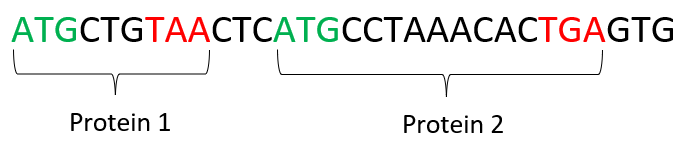
\includegraphics[scale =0.7]{obrazky-figures/proteingener.png}
\caption{Príklad vygenerovanej sekvencie}
\label{generobr}
\end{figure}
\end{theorem}




\chapter{Testovanie}
V nasledujúcej kapitole sa nachádza testovanie a porovnanie výsledkov s webovou aplikáciou Expasy Traslate Tool\footnote{Dostupná na \href{https://web.expasy.org/translate/}{https://web.expasy.org/translate/}} od Swiss Institute of Bioinformatics (SIB). Testovanie je rozdelené do troch častí. V prvej časti je testovaná aplikácia na spracovanie nevalidných vstupných symbolov na vstupe aplikácie ako aj limity vstupu. V druhej časti sú testované parametre aplikácie a ich kombinácie. V závere, a teda poslednej časti testovania, sú výsledky porovnané s výstupom aplikácie Expasy Traslate Tool.

\section{Testovanie vstupu aplikácie}
V tejto časti je aplikácia testovaná na nevalidné znaky vo vstupnej sekvencii. Týmito znakmi sú všetky znaky z ASCII\footnote{Dostupná na \href{http://www.asciitable.com}{http://www.asciitable.com}} tabuľky, okrem znakov nukleotidov a to A, C, T, U ,G. Tie môžu byť zadané malými aj veľkými písmenami latinskej abecedy. Okrem toho prebieha testovanie limit vstupu. Týmito limitami sú maximálna dĺžka generovaného reťazca, ako už bolo spomenuté v sekcii o generovaní \ref{gener} a maximálna dĺžka riadku sekvencie v súbore formátu FASTA.
\section{Testovanie parametrov aplikácie}
V aplikácii sú definované dva druhy parametrov. A to základné a voliteľné. Medzi základné patria:
\begin{itemize}
\item -s: manuálne zadanie vstupnej sekvencie
\item -f: súbor vo formáte FASTA ako vstup aplikácie
\item -h: výpis nápovedy ako používať parametre aplikácie
\item -g -d: vygenerovanie vstupnej DNA sekvencie
\item -g -r: vygenerovanie vstupnej mRNA sekvencie
\end{itemize}
Voliteľnými parametrami sú:
\begin{itemize}
\item -t: výpis tabuľky genetického kódu
\item -c: zadaná vstupná sekvencia je komplementárna
\item -sub: výpis preložiteľných častí sekvencie
\end{itemize}
Voliteľné parametre môžu byť použité v kombinácií so základnými parametrami až na pár výnimiek. Parameter pre nápovedu (-h) nie je použiteľný s ani jedným voliteľným parametrom a parameter generovania nepodporuje voliteľný parameter pre komplementárnu sekvenciu. Na obrázku \ref{priklad1} je zobrazený príklad manuálne zadanej sekvencie a parametru -t. Ako vstupnú sekvenciu využijeme sekvenciu z príkladu \ref{prikladsek} . V prípade generovania, je aplikácia spustená s dodatočným parametrom -sub, ktorý je znázornený na obrázku \ref{priklad2}. Parameter -sub, vo výpise prekladu, vypíše časti vstupnej sekvencie spolu s indexom štart a stop kodónu, ktoré sú aplikáciou preložene na reťazce proteinotvorných aminokyselín. 


\begin{figure}[!hb]
\centering
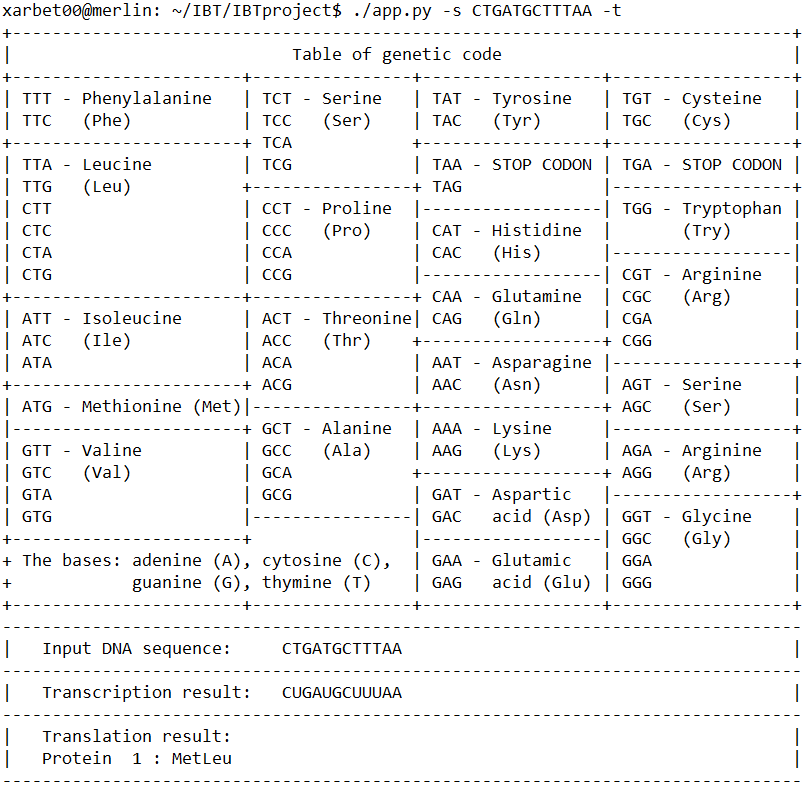
\includegraphics[scale =0.7]{obrazky-figures/priklad1.png}
\caption{Príklad manuálneho zadania vstupnej sekvencie}
\label{priklad1}
\end{figure}


\begin{figure}[!ht]
\centering
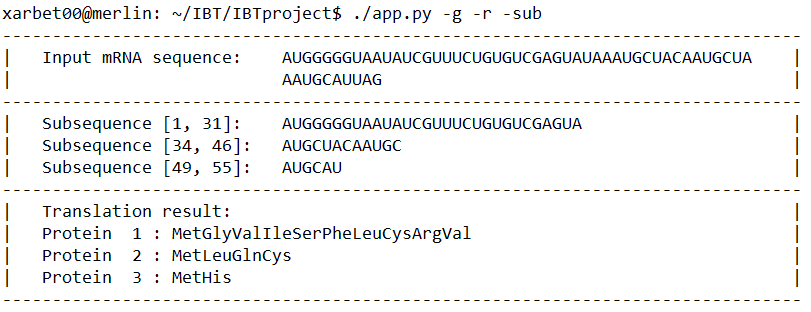
\includegraphics[scale =0.7]{obrazky-figures/priklad2.png}
\caption{Príklad vygenerovania sekvencie mRNA}
\label{priklad2}
\end{figure}



\newpage
\section{Validácia výsledkov aplikácie}
Výsledky aplikácie v procese validácie budú porovnávané už spomenutou aplikáciou Expasy Traslate Tool od Swiss Institute of Bioinformatics (SIB). Ako príklad si vezmeme vygenerovanú sekvenciu \ref{priklad2} z predošlej kapitoly. Výstup referenčnej aplikácie je zobrazený na nasledujúcom obrázku.


\begin{figure}[!ht]
\centering

\includegraphics[scale =0.7]{obrazky-figures/appref.png}
\caption{Výstup aplikácie Expasy Traslate Tool}
\label{priklad3}
\end{figure}



Na prvý pohľad je vidno, že výstupy aplikácii sa líšia. To je spôsobené tým, že aplikácia Expasy Traslate Tool využíva NCBI začnenie, ktoré je znázornené v tabuľke \ref{kodyapp}. Oblasť vyznačená červenou farbou ma význam tzv. Open reading frames. Čo v preklade zamená, časť sekvencie, ktorá je schopná byť preložená. Tá začína, štart kodónom označením ako $M$ a končí stop kodónom označené znakom $-$. Ak do vstupnej aplikácie vložíme kodón, ktorý sa nachádza mimo časť prekladu, aplikácia Expasy Traslate Tool tento kodón preloží. Naša aplikácia tieto kodóny ignoruje. Ako príklad za koniec sekvencie pridáme kodón $GAG$ tak aplikácia to vyhodnotí ako kyselinu glutámovú. Tento výsledok je zobrazený na obrázku \ref{priklad33}

\begin{figure}[!ht]
\centering
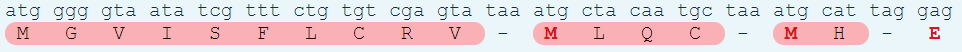
\includegraphics[scale =0.7]{obrazky-figures/appref2.png}
\caption{Výstup aplikácie Expasy Traslate Tool s kodónom navyše}
\label{priklad33}
\end{figure}
\clearpage
\begin{figure}[ht!]
\centering
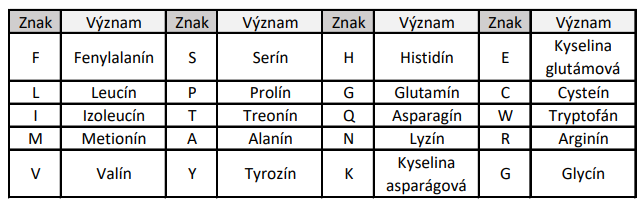
\includegraphics[scale =0.9]{obrazky-figures/kodyapp.png}
\caption{Tabuľka NCBI kódov}
\label{kodyapp}
\end{figure}


\chapter{Záver}
\label{zaver}

TODO.....







  \fi
  
  % Kompilace po částech (viz výše, nutno odkomentovat)
  % Compilation piecewise (see above, it is necessary to uncomment it)
  %\subfile{projekt-01-uvod-introduction}
  % ...
  %\subfile{chapters/projekt-05-conclusion}


  % Pouzita literatura / Bibliography
  % ----------------------------------------------
\ifslovak
  \makeatletter
  \def\@openbib@code{\addcontentsline{toc}{chapter}{Literatúra}}
  \makeatother
  \bibliographystyle{bib-styles/Arbet/skplain}
\else
  \ifczech
    \makeatletter
    \def\@openbib@code{\addcontentsline{toc}{chapter}{Literatura}}
    \makeatother
    \bibliographystyle{bib-styles/Arbet/czplain}
  \else 
    \makeatletter
    \def\@openbib@code{\addcontentsline{toc}{chapter}{Bibliography}}
    \makeatother
    \bibliographystyle{bib-styles/Arbet/enplain}
  %  \bibliographystyle{alpha}
  \fi
\fi
  \begin{flushleft}
  \bibliography{xarbet00-20-literatura-bibliography}
  \end{flushleft}

  % vynechani stranky v oboustrannem rezimu
  % Skip the page in the two-sided mode
  \iftwoside
    \cleardoublepage
  \fi

  % Prilohy / Appendices
  % ---------------------------------------------
  \appendix
%\ifczech
%  \renewcommand{\appendixpagename}{Přílohy}
%  \renewcommand{\appendixtocname}{Přílohy}
%  \renewcommand{\appendixname}{Příloha}
%\fi
\ifslovak
  \renewcommand{\appendixpagename}{Prílohy}
  \renewcommand{\appendixtocname}{Prílohy}
  \renewcommand{\appendixname}{Príloha}
\fi
%  \appendixpage

% vynechani stranky v oboustrannem rezimu
% Skip the page in the two-sided mode
%\iftwoside
%  \cleardoublepage
%\fi
  
\ifslovak
%  \section*{Zoznam príloh}
%  \addcontentsline{toc}{section}{Zoznam príloh}
\else
  \ifczech
%    \section*{Seznam příloh}
%    \addcontentsline{toc}{section}{Seznam příloh}
  \else
%    \section*{List of Appendices}
%    \addcontentsline{toc}{section}{List of Appendices}
  \fi
\fi
  \startcontents[chapters]
  \setlength{\parskip}{0pt} 
  % seznam příloh / list of appendices
  % \printcontents[chapters]{l}{0}{\setcounter{tocdepth}{2}}
  
  \ifODSAZ
    \setlength{\parskip}{0.5\bigskipamount}
  \else
    \setlength{\parskip}{0pt}
  \fi
  
  % vynechani stranky v oboustrannem rezimu
  \iftwoside
    \cleardoublepage
  \fi
  
  % Přílohy / Appendices
  \ifenglish
    \input{xarbet00-30-prilohy-appendices-en}
  \else
    \chapter{Zdrojové kódy, manuál a dokumentácia}

Dostupné na: \url{https://todo}. 

  \fi
  
  % Kompilace po částech (viz výše, nutno odkomentovat)
  % Compilation piecewise (see above, it is necessary to uncomment it)
  %\subfile{projekt-30-prilohy-appendices}
  
\end{document}
